%%%%%%%%%%%%%%%%%%%%%%%%%%%%%%%%%%%%%%%%%
% Beamer Presentation
% LaTeX Template
% Version 1.0 (10/11/12)
%
% This template has been downloaded from:
% http://www.LaTeXTemplates.com
%
% License:
% CC BY-NC-SA 3.0 (http://creativecommons.org/licenses/by-nc-sa/3.0/)
%
%%%%%%%%%%%%%%%%%%%%%%%%%%%%%%%%%%%%%%%%%

%----------------------------------------------------------------------------------------
%	PACKAGES AND THEMES
%----------------------------------------------------------------------------------------

\documentclass{beamer}
\graphicspath{{Figures/}}
\usepackage[utf8]{inputenc}  % Para codificación de texto UTF8.
\usepackage[spanish]{babel}  % Para escritura en castellano.
\usepackage{xcolor}
\usepackage{subfigure}  % Para manejo de subfiguras.
\usepackage{fancybox, graphicx}
\usepackage{array,booktabs}
\usepackage{transparent}
\usepackage[most]{tcolorbox}
\usefonttheme[onlymath]{serif} 
%\usepackage[texcoord,grid,gridunit=mm,gridcolor=red!10,subgridcolor=green!10]
%{eso-pic}
\usepackage[absolute,overlay]{textpos}
\usepackage{tikz}
\usetikzlibrary{arrows.meta, calc, quotes, tikzmark}




\newenvironment<>{varblock}[2][.9\textwidth]{%
	\setlength{\textwidth}{#1}
	\begin{actionenv}#3%
		\def\insertblocktitle{#2}%
		\par%
		\usebeamertemplate{block begin}}
	{\par%
		\usebeamertemplate{block end}%
\end{actionenv}}

\mode<presentation> {

% The Beamer class comes with a number of default slide themes
% which change the colors and layouts of slides. Below this is a list
% of all the themes, uncomment each in turn to see what they look like.

%\usetheme{default}
%\usetheme{AnnArbor}
%\usetheme{Antibes}
%\usetheme{Bergen}
%\usetheme{Berkeley}
%\usetheme{Berlin}
%\usetheme{Boadilla}
\usetheme{CambridgeUS}
%\usetheme{Copenhagen}
%\usetheme{Darmstadt}
%\usetheme{Dresden}
%\usetheme{Frankfurt}
%\usetheme{Goettingen}
%\usetheme{Hannover}
%\usetheme{Ilmenau}
%\usetheme{JuanLesPins}
%\usetheme{Luebeck}
%\usetheme{Madrid}
%\usetheme{Malmoe}
%\usetheme{Marburg}
%\usetheme{Montpellier}
%\usetheme{PaloAlto}
%\usetheme{Pittsburgh}
%\usetheme{Rochester}
%\usetheme{Singapore}
%\usetheme{Szeged}
%\usetheme{Warsaw}

% As well as themes, the Beamer class has a number of color themes
% for any slide theme. Uncomment each of these in turn to see how it
% changes the colors of your current slide theme.

%\usecolortheme{albatross}
%\usecolortheme{beaver}
%\usecolortheme{beetle}
%\usecolortheme{crane}
%\usecolortheme{dolphin}
%\usecolortheme{dove}
%\usecolortheme{fly}
%\usecolortheme{lily}
%\usecolortheme{orchid}
%\usecolortheme{rose}
%\usecolortheme{seagull}
%\usecolortheme{seahorse}
%\usecolortheme{whale}
%\usecolortheme{wolverine}

%\setbeamertemplate{footline} % To remove the footer line in all slides uncomment this line
%\setbeamertemplate{footline}[page number] % To replace the footer line in all slides with a simple slide count uncomment this line

\setbeamertemplate{navigation symbols}{} % To remove the navigation symbols from the bottom of all slides uncomment this line
}

\usepackage{graphicx} % Allows including images
\usepackage{booktabs} % Allows the use of \toprule, \midrule and \bottomrule in tables
\renewcommand{\vec}[1]{\boldsymbol{#1}}
%----------------------------------------------------------------------------------------
%	TITLE PAGE
%----------------------------------------------------------------------------------------

\title[Tesis de grado]{Estudio de estructuras de banda prohibida electromagnética (EBG) para la reducción de acoplamiento mutuo entre antenas \textit{microstrip}} % The short title appears at the bottom of every slide, the full title is only on the title page

\author{Federico Luna} % Your name
\institute[] % Your institution as it will appear on the bottom of every slide, may be shorthand to save space
{
Facultad de Ingeniería,\\
Universidad de Buenos Aires \\ % Your institution for the title page
\medskip
\textit{fluna@fi.uba.ar}\\
\medskip % Your email address
Tutores: Dr. Ing. W. Gustavo Fano y Mg. Ing. Silvina Boggi
}
\date{} % Date, can be changed to a custom date

\begin{document}

	\begin{frame}
		\titlepage % Print the title page as the first slide
	\end{frame}

\begin{frame}
\frametitle{Resumen} % Table of contents slide, comment this block out to remove it
\tableofcontents[hideallsubsections] % Throughout your presentation, if you choose to use \section{} and \subsection{} commands, these will automatically be printed on this slide as an overview of your presentation
\end{frame}

%----------------------------------------------------------------------------------------
%	PRESENTATION SLIDES
%----------------------------------------------------------------------------------------

%------------------------------------------------
\section{Presentación del problema} % Sections can be created in order to organize your presentation into discrete blocks, all sections and subsections are automatically printed in the table of contents as an overview of the talk
%------------------------------------------------
		\begin{frame}
			\frametitle{Objetivo}
			
			\begin{itemize}
				\item Propagación de ondas de superficie.
				\item Estructuras periódicas.
				\item Comportamiento de EBGs uniplanares.
				\item Modelo circuital equivalente de una celda unitaria.
				\item Programa de simulación en el dominio del tiempo.
				\item Introducción al uso de EBGs en conjuntos de antenas.
			\end{itemize}
		\end{frame}
	
		\begin{frame}
		\frametitle{Reseña histórica}
		\begin{itemize}
			\item 1873: \textbf{Maxwell}. Bases de teoría electromagnética clásica.\\
			\item 1885-1887: \textbf{Heaviside}. Simplificación de expresiones: Notación vectorial. \\
			\item 1886-1891: \textbf{Hertz}. Validación de teoría de ondas electromagnéticas. Primer antena dipolo y parabólica.
			\item 1897: \textbf{Rayleigh}. Propagación de ondas en guías metálicas.
			\item 1926: \textbf{Yagi-Uda}. Conjunto de antenas, fase fija.
			\item 1938-1945: Antenas de fase variable.
			\item 1953: \textbf{Deschamps}. Antenas \textit{microstrip}.
			\item 1970': Uso en aplicaciones prácticas. Solución a problemas de dispersión y modos indeseados.
			% Sustratos con bajas tangentes de pérdida. Mejora en fotolitografía. Optimización de modelos teóricos, simulaciones numéricas. Simplificación constructiva, más barato.
		\end{itemize}
		\end{frame}
	
		\begin{frame}
		\frametitle{Ventajas de las estructuras \textit{microstrip}}
		
		\begin{columns}[c] % The "c" option specifies centered vertical alignment while the "t" option is used for top vertical alignment
			
			\column{.50\textwidth} % Left column and width
			\begin{figure}[h]
				\centering
				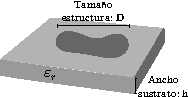
\includegraphics[width=1\textwidth]{Presentacion/microstrip_general.pdf}
			\end{figure}
			
			\column{.45\textwidth} % Right column and width
			\begin{itemize}
				\item Bajo \textbf{costo}.
				\item Bajo \textbf{peso}.
				\item \textbf{Construcción} sencilla (fotolitografía).
				\item Cómodas para implantación de \textbf{componentes discretos}.
				\item Alto \textbf{Q} (resonantes).
			\end{itemize}
		
		\end{columns}
	
	\vspace{25pt}
	
	\centering Aplicaciones: filtros microondas, acopladores direccionales, transformadores de impedancia, planos de tierra y redes de distribución de circuitos impresos.
		
	\end{frame}
		
		\begin{frame}
			\frametitle{Problemas de las estructuras \textit{microstrip}}
			\begin{itemize}
				\item Alto \textbf{Q}.
				\item Difícil \textbf{estudio analítico}.
				\begin{itemize}
					\item Modos superiores.
					\item Lóbulos secundarios en antenas.
					\item Efectos de borde.
				\end{itemize}
				\item Baja \textbf{eficiencia}.
				\item Polarización impura.
				\item \textbf{Fragilidad}.
				\item \textbf{Tamaño} proporcional a las frecuencias de trabajo.
				\item {\color{red}\textbf{Acoplamiento mutuo} con estructuras cercanas.}
				\begin{itemize}
					\item Acoplamiento por campo cercano.
					\item Acoplamiento por red de alimentación compartida.
					\item {\color{red}Acoplamiento por \textbf{ondas de superficie} con otras estructuras con las que comparte plano de tierra.}
				\end{itemize}
			\end{itemize}
		
			\pause
			
			\begin{textblock*}{65mm}(65mm,12mm)
				\includegraphics<2>[width=1\textwidth]{Presentacion/problema_microstrip2.pdf}
			\end{textblock*}
		\end{frame}
	

		
		
		% Acá la idea es comentar que en general uno busca disminuir el tamaño. Eempezando de la esquina inferior derecha, uno tiene una estructura grande y fuerte. La quiere achicar, sale de la zona verde, hay mas ondas de superficie, y para bajar esas ondas no queda otra que bajar el ancho del sustrato, generando mayor fragilidad estructural. Modos indeseados.
		\begin{frame}
		\frametitle{Soluciones propuestas en la literatura}
		
		\begin{itemize}
			\item \textbf{Separación del plano de tierra} de las estructuras.
			\item \textbf{Modificar la altura} o la permitividad del sustrato a corta distancia.
			\item \textbf{Estructuras periódicas}: EBG, DGS.
		\end{itemize}
		
		\begin{figure}[H]
			\centering 
			\subfigure{
				\label{fig:sustrato-antena-ebg}
				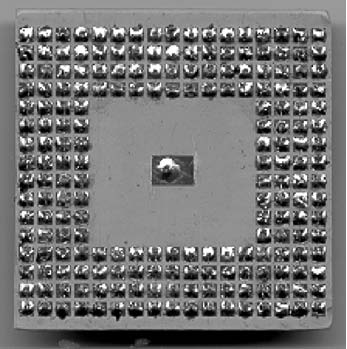
\includegraphics[width=0.40\textwidth]{Aplicacion/foto-ebg-alrededor-antena.pdf}}
			\hspace{10pt}
			\subfigure{
				\label{fig:escalon-sustrato}
				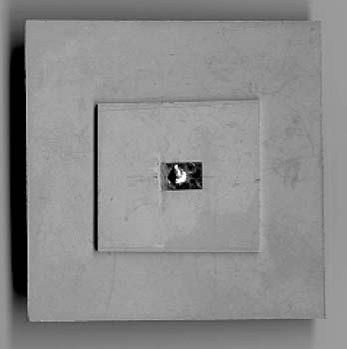
\includegraphics[width=0.40\textwidth]{Aplicacion/foto-escalon-alrededor-antena.pdf}}
		\end{figure}
		\tiny{F. Yang e Y. Rahmat-Samii, Electromagnetic Band Gap Structures in Antenna Engineering, Cambridge University Press, 2009.}
		\end{frame}

\section{Conceptos básicos de electromagnetismo}
	
	
	\begin{frame}
		\frametitle{Conceptos básicos de electromagnetismo}
		\tableofcontents[currentsection,hideothersubsections]
	\end{frame}
	
	\subsection{Ecuaciones de Maxwell y ondas electromagnéticas} % A subsection can be created just before a set of slides with a common theme to further break down your presentation into chunks
	
		\begin{frame}
			\frametitle{Ecuaciones de Maxwell}
			
			\begin{align*}
			\left.\begin{array}{rr@{\mskip\thickmuskip}l}
			\text{Faraday} &\nabla \times \vec{E} & = -\frac{\partial \vec{B}}{\partial t} - \vec{M}\\
			\text{Ampère} &\nabla \times \vec{H} & = \frac{\partial \vec{D}}{\partial t} + \vec{J} \\
			\text{Gauss} &\nabla \cdot \vec{D} & = \rho \\
			\text{Gauss} & \nabla \cdot \vec{B} & = 0
			\end{array} \right\}
			\quad \implies \quad
			\left\{\begin{array}{r@{\mskip\thickmuskip}l}
			\nabla \times \vec{E} & = -j \omega \vec{B} - \vec{M} \\
			\nabla \times \vec{H} & = j \omega \vec{D} + \vec{J} \\
			\nabla \cdot \vec{D} & = \rho\\
			\nabla \cdot \vec{B} & = 0
			\end{array}\right.
			\end{align*}
			
			\begin{textblock*}{18mm}(62mm,25mm)
				\tiny \centering Sin dispersión,
				isotrópico,
				armónico,\\
				rég. perm.
			\end{textblock*}
			
			\begin{columns}[c]
				\column{0.8\textwidth}
				\begin{align*}
					\vec{D} &= \epsilon_0 \vec{E} + \vec{P}_e = \epsilon_0 (1+\chi_e)\vec{E} = \epsilon \vec{E} = (\epsilon' - j \epsilon'') \vec{E}\\
					\vec{B} &= \mu_0 (\vec{H} + \vec{P}_m) = \mu_0 (1+\chi_m)\vec{H} = \mu \vec{H} = (\mu' - j \mu'') \vec{H}.
				\end{align*}
				\column{0.05\textwidth}
			\end{columns}
		
			\begin{textblock*}{15mm}(110mm,55mm)
				\tiny \centering Medio\\
				lineal,\\
				isotrópico\\
				homogéneo.
			\end{textblock*}
			
			\vspace{0.7cm}
			\begin{align*}
			\vec{J} &= \sigma \vec{E} \Rightarrow \vec{D} = \left( \epsilon' - j\epsilon'' - j \frac{\sigma}{\omega} \right) \vec{E}.
			\end{align*}
			
			\begin{textblock*}{24mm}(8mm,77mm)
				\scriptsize \centering $\sigma$
				indep. del
				campo aplicado: \textbf{Ohm}.
			\end{textblock*}		
		
		\end{frame}
			

		\begin{frame}
			\frametitle{Ondas electromagnéticas (I)}
			
			\begin{figure}[h]
				\centering
				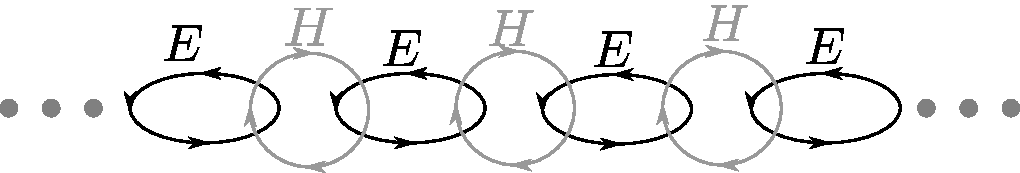
\includegraphics[width=1\textwidth]{Presentacion/onda_em.pdf}
			\end{figure}
			
			\centering \textbf{Ecuaciones de Helmholtz}
					
			\begin{align*}
			\left.\begin{array}{rr@{\mskip\thickmuskip}l}
			\nabla^2  \vec{E} + \gamma^2 \vec{E} &= 0\\
			\nabla^2 \vec{H} + \gamma^2 \vec{H}& = 0
			\end{array} \right\}
			\quad \implies \quad
			\left\{\begin{array}{r@{\mskip\thickmuskip}l}
			\vec{E}(x,y,z) &= \vec{E}_0 e^{\pm j \vec{\gamma}\cdot \vec{r}}. \\
			\vec{H}(x,y,z) &= \vec{H}_0 e^{\pm j \vec{\gamma}\cdot \vec{r}}.
			\end{array}\right.
			\end{align*}
			
			\begin{columns}[c]
				\column{0.6\textwidth}
				\begin{block}{}
					\setlength\abovedisplayskip{0pt}
					\begin{align*}
					\centering
					\gamma &= -j\alpha + \beta = j\omega \sqrt{\mu (\epsilon'-j\epsilon'') - j \sigma \epsilon/\omega}
					\end{align*}
				\end{block}
				\column{0.3\textwidth}
				\begin{block}{}
					\setlength\abovedisplayskip{0pt}
					\begin{align*}
					\centering \vec{\gamma} &= \vec{\gamma}_x + \vec{\gamma}_y +\vec{\gamma}_z
					\end{align*}
				\end{block}
			\end{columns}
		
			\begin{block}{}
				\setlength\abovedisplayskip{0pt}
				\begin{align*}
				E_i(z) = E_i \; e^{-j\gamma z} = E_i \; {\color{red}e^{-\alpha z}} \; {\color{violet}e^{-j \beta z}}, \quad i=x,y.
				\end{align*}
			\end{block}

		\end{frame}
	
		\begin{frame}
			\frametitle{Ondas electromagnéticas (II)}
			
			Para las ondas planas,
			
			\begin{block}{}
				\setlength\abovedisplayskip{0pt}
				\begin{align*}
				\vec{H}(\vec{r},t) &= \pm \frac{\hat{\beta} \times \vec{E}(\vec{r},t)}{\eta}.
				\end{align*}
			\end{block}
		
		
		
			\begin{columns}[c] % The "c" option specifies centered vertical alignment while the "t" option is used for top vertical alignment
				
				\column{.45\textwidth} % Left column and width
				
				\begin{block}{\centering Impedancia de onda}
					\setlength\abovedisplayskip{0pt}
					\begin{align*}
					\eta &= \frac{j \omega \mu}{\gamma }.
					\end{align*}
				\end{block}
			
				\begin{block}{\centering Velocidad de fase}
					\setlength\abovedisplayskip{0pt}
					\begin{align*}
					v_p &= \omega/\beta = c/\sqrt{\mu_r \epsilon_r}.
					\end{align*}
				\end{block}
			
				
				
				\column{.45\textwidth} % Right column and width
				
				\begin{block}{\centering Prof. penetración}
					\setlength\abovedisplayskip{0pt}
					\begin{align*}
					\label{eq:prof_penetacion}
					\delta_s = -1/\alpha &= \sqrt{\frac{2}{\omega \mu \sigma}}.
					\end{align*}
				\end{block}
			
				\begin{block}{\centering Velocidad de grupo}
					\setlength\abovedisplayskip{0pt}
					\begin{align*}
					v_g &= d\omega/d\beta.
					\end{align*}
				\end{block}
			
			\end{columns}
			
			

		\end{frame}
		
		\subsection{Antenas}
		
		\begin{frame}
			\frametitle{Fuentes de ondas electromagnéticas: Antenas}
			\begin{block}{Antena}
				\centering
				Interfaz para las ondas electromagnéticas entre el espacio libre y un dispositivo de guía, generalmente metálico.\\
				\textbf{Objetivo}: Recibir y transmitir energía eficientemente.
			\end{block}
				
			\begin{block}{}
				Se suelen utilizar en conjuntos radiantes, dispuestas geométricamente.
			\end{block}
			
			\centering	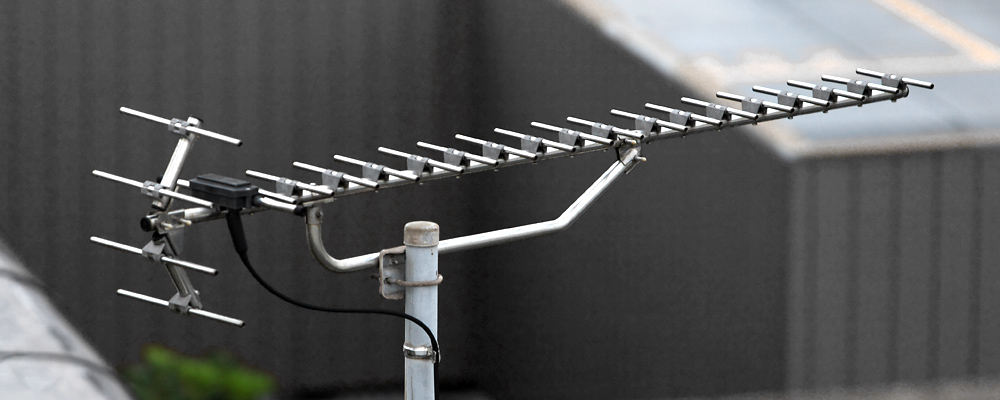
\includegraphics[width=0.7\textwidth]{Presentacion/yagi-uda.JPG}

		\end{frame}
		
		\begin{frame}
			\frametitle{Acoplamiento entre antenas \textit{microstrip}}
			\begin{block}{Responsables}
				\begin{itemize}
					\centering
					\item Acoplamiento espacial entre elementos por \textbf{onda espacial} ($\downarrow \propto 1/\rho$).
					\item Acoplamiento espacial por \textbf{onda de superficie} ($\downarrow \propto 1/\sqrt\rho$).
					\item Acoplamiento por \textbf{red de alimentación} (alimentación no independiente).
				\end{itemize}
			\end{block}
			
			
			\begin{columns}[c]
				\centering
				\column{0.6\textwidth}
					\begin{align*}
						\begin{bmatrix}
						V_1 \\ V_2 \\ \vdots \\ V_N
						\end{bmatrix}
						=
						\underbrace{\begin{bmatrix}
							Z_{11} & Z_{12} & \cdots & Z_{1N} \\
							Z_{12} & Z_{22} & \cdots & Z_{2N} \\
							\vdots & \vdots & \cdots & \vdots \\
							Z_{1N} & Z_{2N} & \cdots & Z_{NN} \\
							\end{bmatrix}}_{Z}
						\begin{bmatrix}
						I_1 \\ I_2 \\ \vdots \\ I_N
						\end{bmatrix}
					\end{align*}
				\column{0.4\textwidth}
				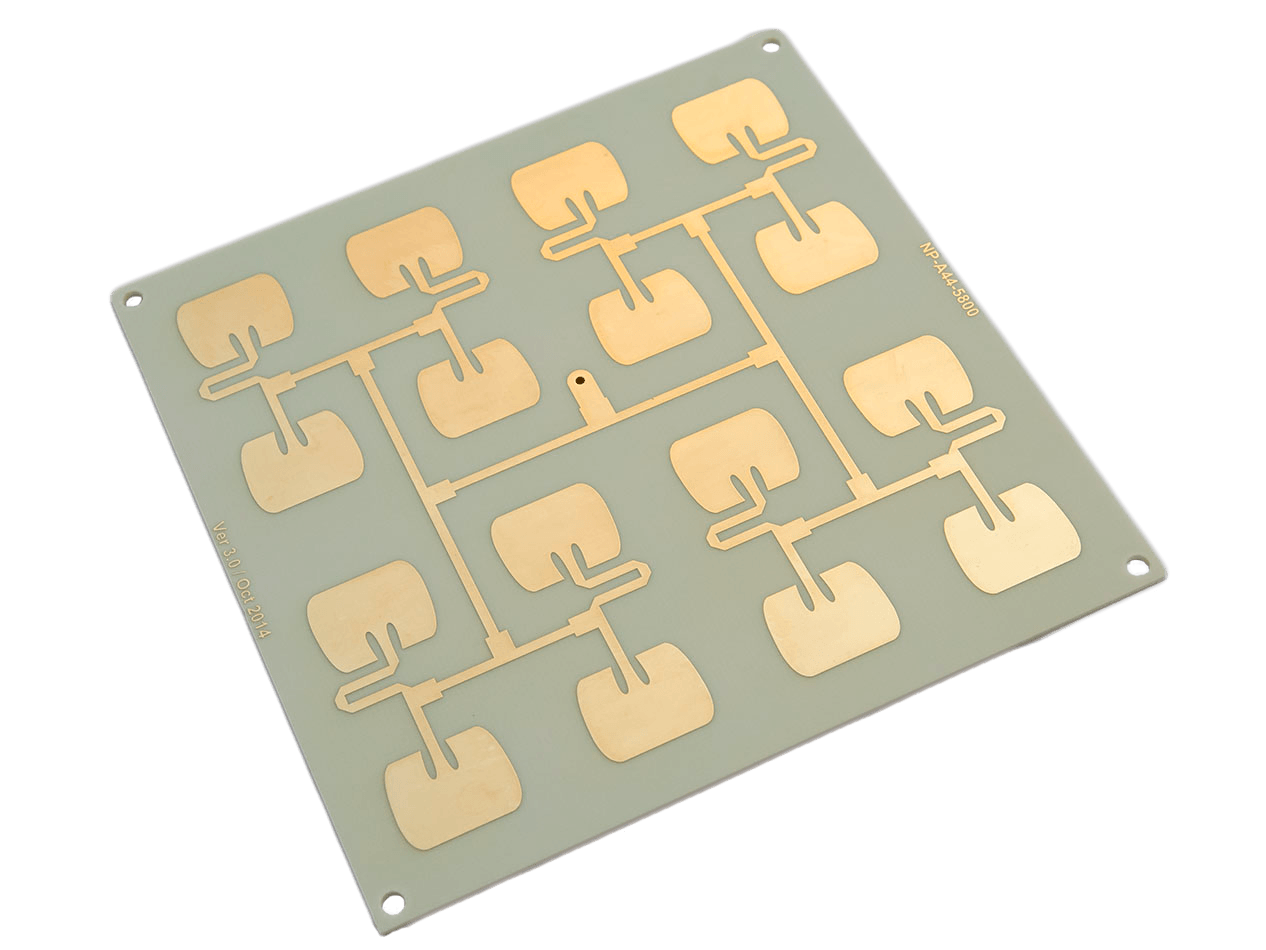
\includegraphics[width=\textwidth]{Presentacion/arregloMicrostrip.png}
			\end{columns}
			
					
		\end{frame}
		
		
		% Comparar Masters Eq con Shrodinger. Modos.
		\subsection{Ondas de superficie}
		
			\begin{frame}
			\frametitle{Ondas de superficie}
			
			\begin{block}{}
				\centering
				Se propagan en un plano.
				
				Comportamiento evanescente en la dirección normal.
			\end{block}
			
			\begin{figure}[]
				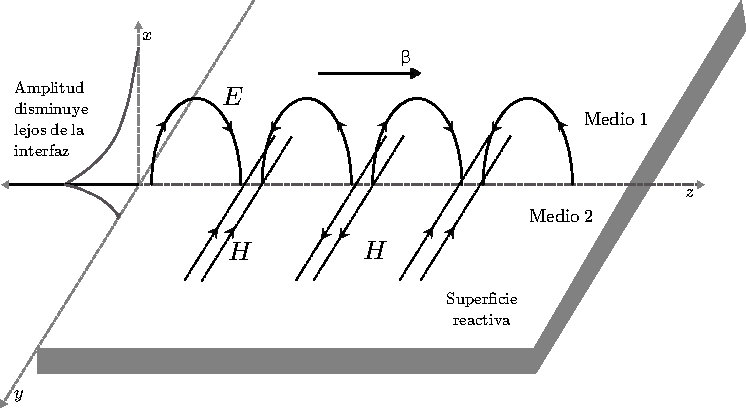
\includegraphics[width=0.60\textwidth]{intro_electro/ondas-superficie-3d.pdf}
			\end{figure}
		
			\begin{columns}[c] % The "c" option specifies centered vertical alignment while the "t" option is used for top vertical alignment
				
				\column{.55\textwidth}
				\begin{itemize}
					\centering
					\item Planos conductores.
					\item Planos conductores recubiertos de dieléctrico.
				\end{itemize}
				\column{.51\textwidth}

				\begin{itemize}
					\centering
					\item Planos corrugados.
					\item Interfaz entre dos medios distintos.
				\end{itemize}
			\end{columns}
		
			\begin{textblock*}{24mm}(95mm,55mm)
				\small \centering Uller, Zenneck, Sommerfeld, Dyakonov, etc.
			\end{textblock*}
			
			\end{frame}
	
			\begin{frame}
			\frametitle{Ondas de Zenneck}
			
			\begin{columns}[c] % The "c" option specifies centered vertical alignment while the "t" option is used for top vertical alignment
				\column{.42\textwidth}
				\begin{itemize}
					\item TM.
					\item Bajas pérdidas.
					\item Ángulo de Brewster: $Z_1 = Z_2$
				\end{itemize}
			
				
				\begin{align*}
				Z_1 = \frac{{E_z}_1}{{H_y}_1} = \eta_0 \cos\; \theta_i = \frac{\gamma_{x_1}}{\gamma_1} \eta_0\\
				Z_2 = \frac{{E_z}_2}{{H_y}_2} = \eta_2 \cos \; \theta_t = \frac{\gamma_{x_2}}{\gamma_2} \eta_2
				\end{align*}
				
				\begin{block}{}
					\centering
				$\gamma$ a uno y otro lado de la interfaz es complejo.
				\end{block}
			
				\column{.6\textwidth}
				
				\begin{figure}
					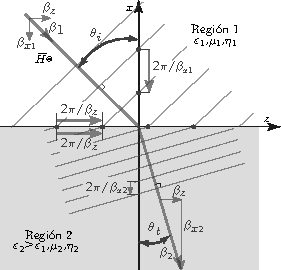
\includegraphics[width=\textwidth]{intro_electro/onda-superficie-incidencia-brewster.pdf}
				\end{figure}
			\end{columns}
			
			\end{frame}
		
			\begin{frame}
				\frametitle{Impedancia de superficie y constante de propagación (TM)}
				
				\centering Si se asume una impedancia de superficie $Z_s = R_s + j X_s$, al igualar la impedancia de onda a la de superficie:
				
				\begin{block}{TM}
				\setlength\abovedisplayskip{0pt}
				\begin{align*}
					\gamma_{x_1} & = \gamma_1 \frac{Z_1}{\eta_0} = \gamma_1 Z_s = \gamma_1 R_s + j \gamma_1 X_s\tikzmark{x1},\\
					\gamma_z &= \beta_z - j\alpha_z =\sqrt{(\gamma_1^2 - \gamma_{x_1}^2)} = \gamma_1 \sqrt{1+X_s^2\tikzmark{x5} - R_s^2 {\color{red}-} 2jR_s X_s\tikzmark{x3}}.
				\end{align*}
				\end{block}
			
				\only<1,2,3,4>{
				\begin{columns}[c]
					\column{.48\textwidth}
					\begin{itemize}
						\item $X_s > 0$: Reactancia inductiva:
						\begin{itemize}
							\item $\uparrow \alpha_x$: Decrecimiento exponencial en $x$\tikzmark{x0}.\\
							\item $\alpha_z > 0$: Decrecimiento exponencial en $z$.\tikzmark{x2}
							\item $\uparrow \beta_z$, $\downarrow v_p$.\tikzmark{x4}
						\end{itemize}
					\end{itemize}
				
					\column{.44\textwidth}
					\begin{itemize}
						\item Si $R_s X_s$ es pequeño: Baja\tikzmark{x6} atenuación en $z$.
					\end{itemize}
					
					\begin{block}{}
						\centering
						Para ondas de superficie TM:
						\centering
						$\uparrow X_s \qquad \downarrow R_s$.

					\end{block}
				\end{columns}
				}
				\only<2>{
					\begin{tikzpicture}[overlay,remember picture]
						\draw[very thick, -Stealth]         ($({pic cs:x0})+(1ex,1ex)$)
						to [bend right, sloped]  ($({pic cs:x1})+(-1ex,-0.5em)$);
					\end{tikzpicture}
				}
			
				\only<3>{
					\begin{tikzpicture}[overlay,remember picture]
					\draw[very thick, -Stealth]         ($({pic cs:x2})+(1ex,1ex)$)
					to [bend right, sloped]  ($({pic cs:x3})+(-1ex,-0.5em)$);
					\end{tikzpicture}
				}
			
				\only<4>{
					\begin{tikzpicture}[overlay,remember picture]
					\draw[very thick, -Stealth]         ($({pic cs:x4})+(1ex,1ex)$)
					to [bend left, sloped]  ($({pic cs:x5})+(-3ex,0em)$);
					\draw[very thick, -Stealth]         ($({pic cs:x6})+(1ex,1ex)$)
					to [bend right, sloped]  ($({pic cs:x3})+(-1ex,-0.5em)$);
					\end{tikzpicture}
				}
			
				\only<5>{\begin{block}{TE}
					\setlength\abovedisplayskip{0pt}
					\begin{align*}
					\gamma_{x_1} &= -\frac{\gamma_1}{Z_s} = -\gamma_1 \frac{R_s}{{\color{red}R_s^2+X_s^2}}-j\frac{X_s}{{\color{red}R_s^2+X_s^2}},\\
					\gamma_z &= \beta_z-j\alpha_z= \sqrt{(\gamma_1^2 - \gamma_{x_1}^2)} = \frac{\gamma_1}{{\color{red}R_s^2+X_s^2}} \sqrt{1+X_s^2 - R_s^2 {\color{red}+} 2jR_s X_s}.
					\end{align*}
				\end{block}
			
				\begin{textblock*}{40mm}(80mm,30mm)
					\begin{block}{\centering Condiciones TM}
						\centering
						$\uparrow X_s \qquad \downarrow R_s$.
					\end{block}
				\end{textblock*}
			
				\begin{textblock*}{40mm}(80mm,60mm)
					\begin{block}{\centering Condiciones TE}
						\centering
						$\downarrow X_s \qquad \downarrow R_s$.
						
					\end{block}
				\end{textblock*}
				}
	
			\end{frame}
		
			\begin{frame}
				\only<1>{\begin{figure}[htp]
					\centering
					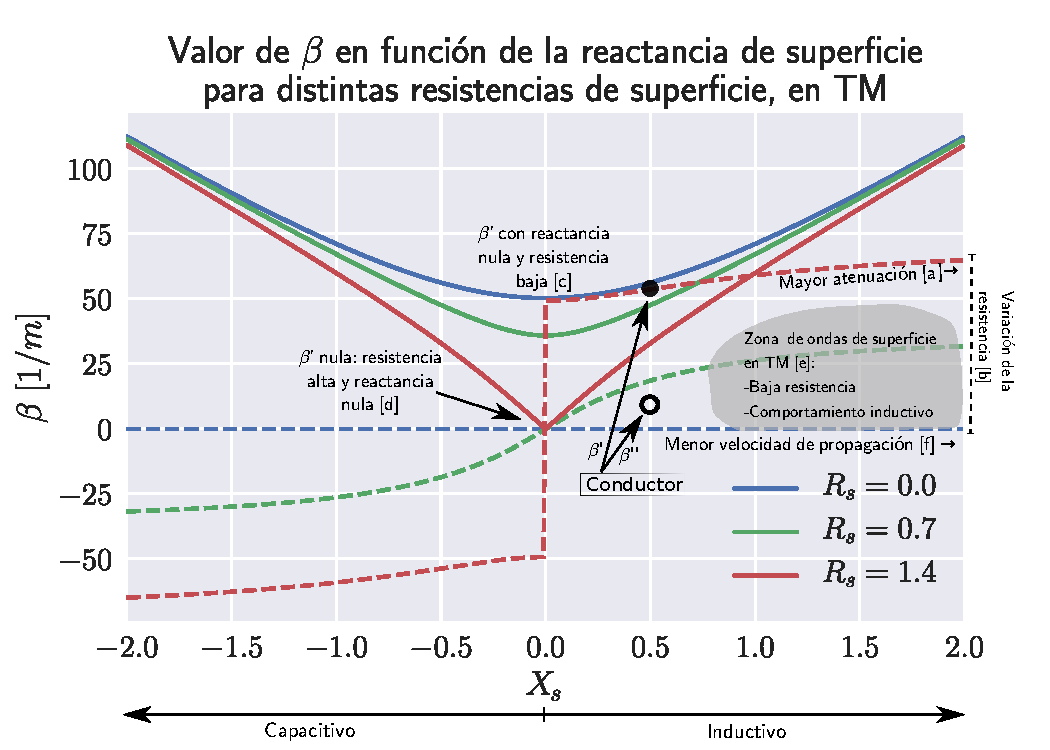
\includegraphics[width=\textwidth]{intro_electro/plot-beta-reactancia-TM.pdf}
				\end{figure}}
			
				\only<2>{\begin{figure}[htp]
					\centering
					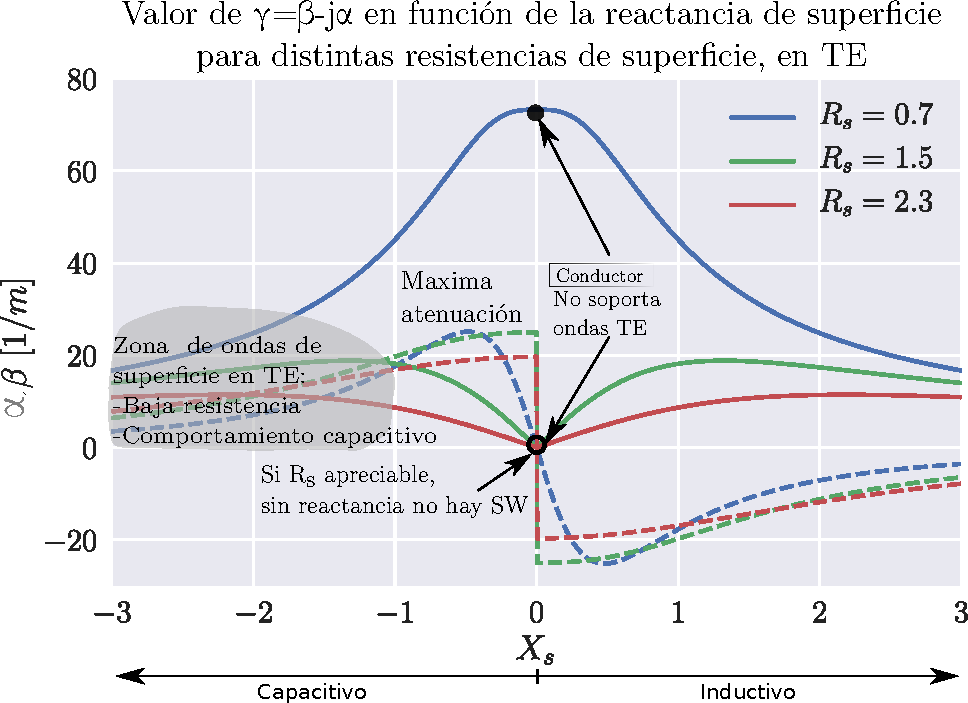
\includegraphics[width=\textwidth]{intro_electro/plot-beta-reactancia-TE.pdf}
				\end{figure}}
			\end{frame}
		
		\begin{frame}
		\frametitle{Condiciones para la propagación sobre un plano conductor}
		
			\begin{block}{\centering Polarización TM}
				\begin{itemize}
					\centering
					\item Comportamiento {\color{red} inductivo}.
					\item Resistividad baja.
				\end{itemize}
			\end{block}
			\begin{block}{\centering Polarización TE}
				\begin{itemize}
					\centering
					\item Comportamiento {\color{red} capacitivo}.
					\item Resistividad baja.
				\end{itemize}
			\end{block}
		
			\centering Para volver más inductiva a la superficie, se puede recubrir al plano conductor con un dieléctrico.
		\end{frame}
	
		\begin{frame}
			\frametitle{Comportamiento para plano de tierra cubierto por un dieléctrico fino}
			\begin{figure}[h]
				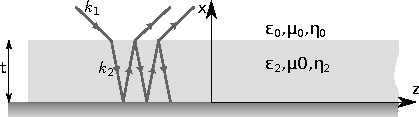
\includegraphics[width=\textwidth]{intro_electro/incidencia-coated-conductor.pdf}
			\end{figure}
		
			\begin{columns}[c]
				\column{.54\textwidth}
				\centering Caso TM:
				
				\begin{align*}
					\begin{cases}
						(\gamma_{x_2} h)^2 + (\alpha_{x_1} h)^2 = (\epsilon_{r_2} - 1) (\gamma_1 h)^2\\
						\gamma_{x_2} h \tan (\gamma_{x_2} h) = |\alpha_{x_1}| \epsilon_{r_2} h.
					\end{cases}
				\end{align*}
				
				\column{.45\textwidth}
				\centering Caso TE:
				
				\begin{align*}
					\begin{cases}
						(\gamma_{x_2} h)^2 + (\alpha_{x_1} h)^2 = (\epsilon_{r_2} - 1) (\gamma_1 h)^2 \\
						\gamma_{x_2} h \cot (\gamma_{x_2} h) = -|\alpha_{x_1}| \epsilon_{r_2} h.
					\end{cases}
				\end{align*}
	
			\end{columns}
		\end{frame}
		
		\begin{frame}
			\begin{columns}[c]
				\column{.52\textwidth}
				\centering TM
					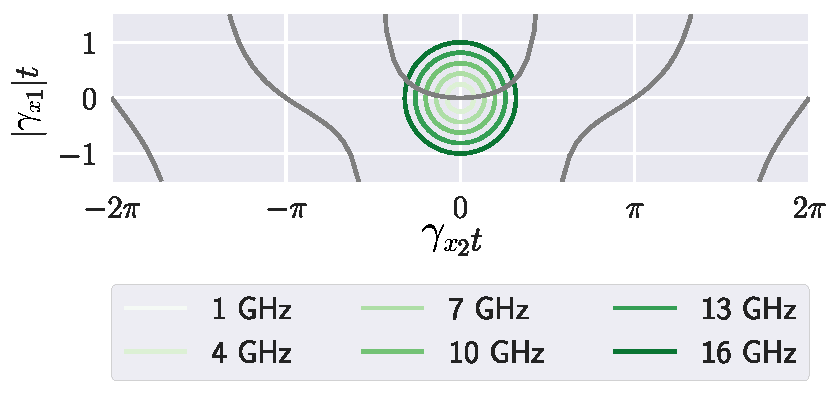
\includegraphics[width=\textwidth]{intro_electro/TM-tan-implicito}
					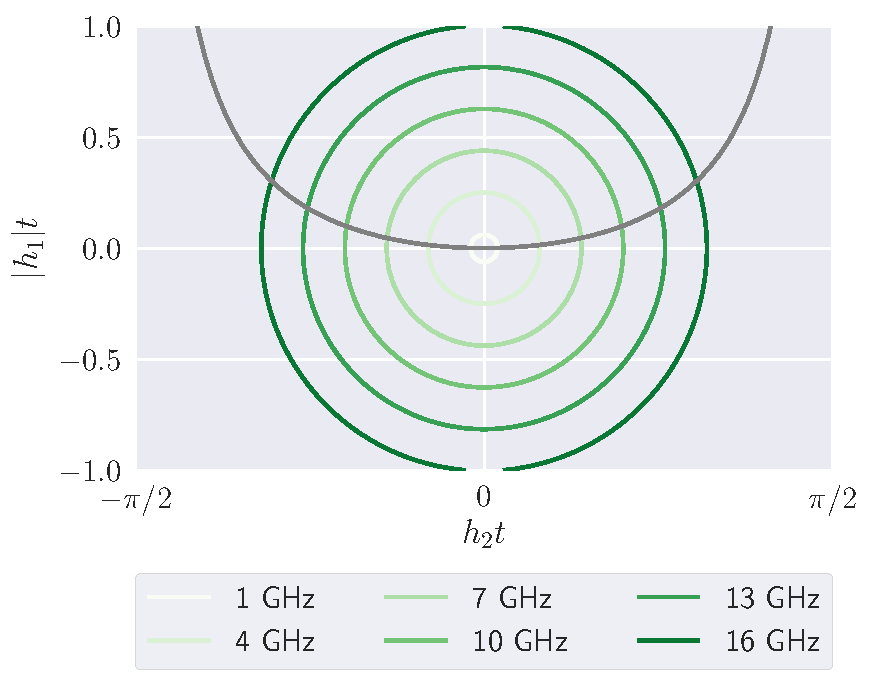
\includegraphics[width=\textwidth]{intro_electro/TM-tan-implicito-zoom}
				
				\column{.52\textwidth}
				\centering TE
					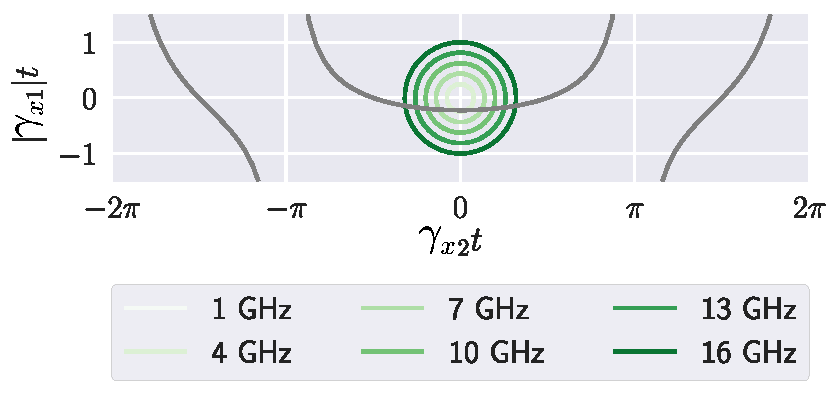
\includegraphics[width=\textwidth]{intro_electro/TE-tan-implicito}
					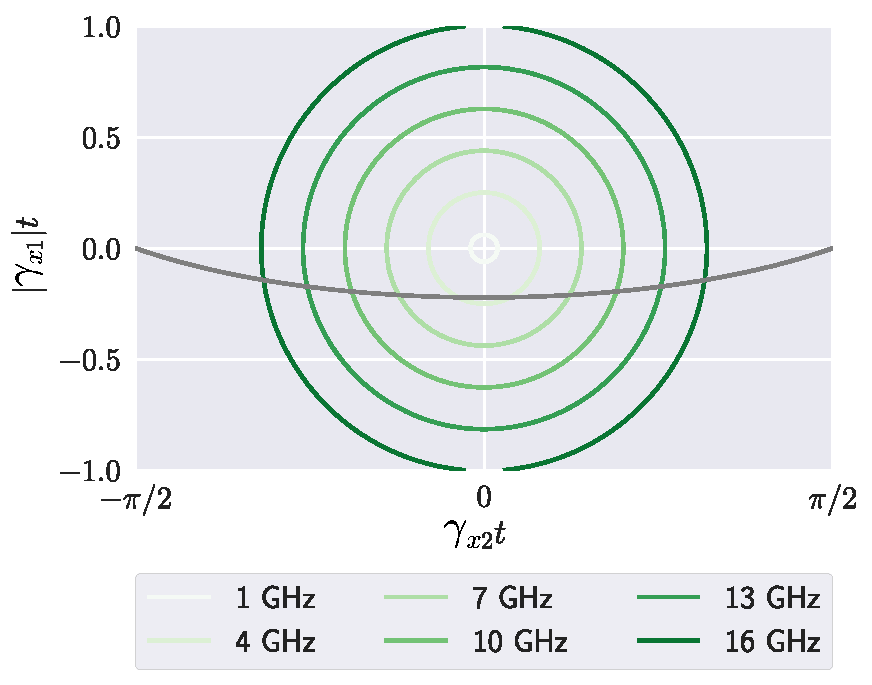
\includegraphics[width=\textwidth]{intro_electro/TE-tan-implicito-zoom}
			\end{columns}
		\end{frame}
	
	
		\begin{frame}
			\frametitle{Impedancia de superficie: GND+FR4}
			\begin{align*}
				Z_s^{TM} = j \frac{\cos \theta_t}{\sqrt{\epsilon_{r_2}}}\tan(\gamma_2 h \cos\theta_t) = j \frac{\cos \theta_t}{\sqrt{\epsilon_{r_2}}}\tan(	\omega\sqrt{\epsilon_{r_2} \mu_0 \epsilon_0} h \cos\theta_t)
			\end{align*}
		
			\begin{columns}[c]
				\column{.51\textwidth}
					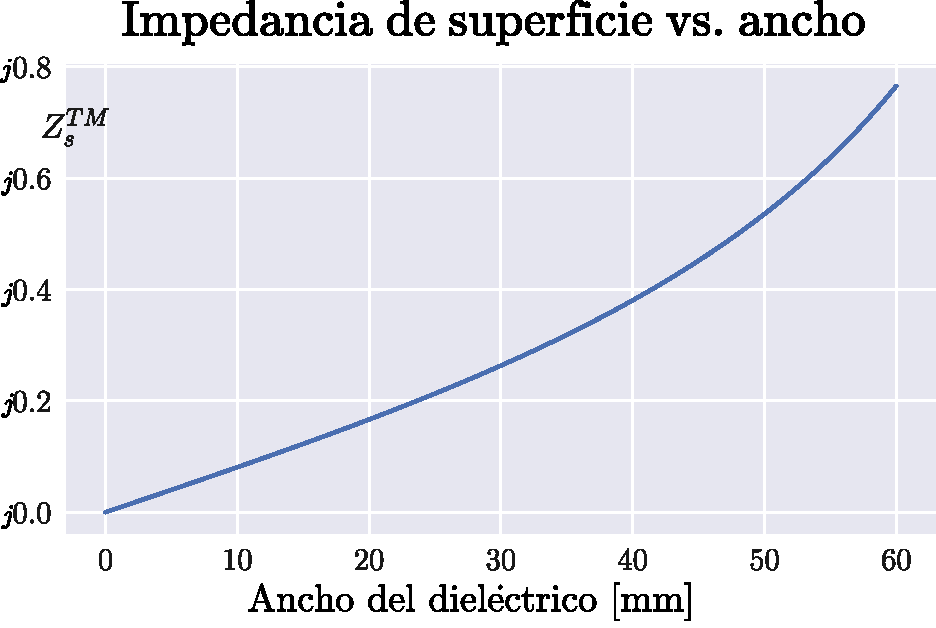
\includegraphics[width=\textwidth]{intro_electro/plot-zstm-funciont2.pdf}
				\column{.51\textwidth}
					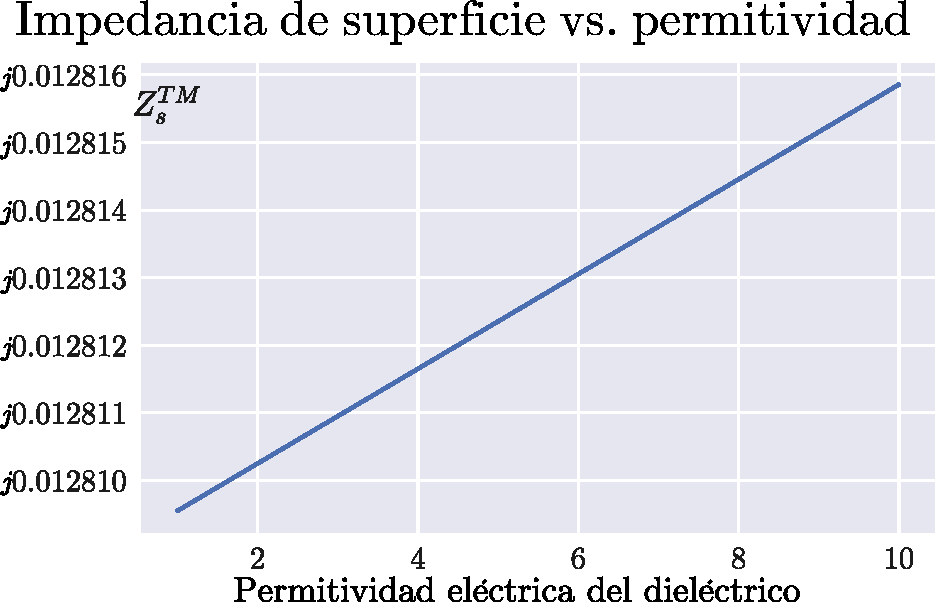
\includegraphics[width=\textwidth]{intro_electro/plot-zstm-funcioner2.pdf}
				
			\end{columns}
			\centering A más alta la impedancia de superficie, mayor incidencia de ondas de superficie.
		\end{frame}
	
		\begin{frame}
			\frametitle{En resúmen}
			\begin{block}{}
				\centering
				No existirán ondas de superficie de polarización TE en el plano de tierra recubierto por 1.6 mm de espesor de FR4, hasta los 25 GHz.
			\end{block}
		
			\begin{block}{}
				\centering
				$\uparrow \text{ancho del sustrato} \Rightarrow\; \uparrow$ ondas de superficie (TM)
			\end{block}
			
			\begin{block}{}
				\centering
				$\uparrow \text{permitividad eléctrica del sustrato} \Rightarrow\; \uparrow$ ondas de superficie (TM)
			\end{block}
		\end{frame}
		
		\subsection{Antenas \textit{microstrip}}
		
		\begin{frame}
			\frametitle{Antenas \textit{microstrip}}
			\begin{columns}[t]
				\column{.45\textwidth} % Right column and width
					\color{red}Alto acoplamiento con elementos ubicados sobre la superficie.
					\begin{block}{}
						\centering
						$\uparrow \epsilon_r \Rightarrow$\\ $\uparrow$ acoplamiento,\\$\downarrow$ pot. radiada,\\ $\uparrow$ lóbulos secundarios.
					\end{block}
					\vspace{0.5cm}
					\begin{itemize}
						\item $\downarrow D \Rightarrow \uparrow \epsilon_r,$ {\color{red}$\uparrow$ SW}.
						\item $\uparrow \epsilon_r \Rightarrow \uparrow Q, \downarrow$ BW.
						\item $\downarrow Q \Rightarrow \uparrow h$.
						\item $\uparrow h \Rightarrow ${\color{red}$\uparrow$ SW}, $\uparrow$ modos.
					\end{itemize}
				
				\column{.50\textwidth} % Right column and width
					\color{red}Bajo acoplamiento con elementos cercanos. Campos contenidos en el sustrato.
					\begin{block}{}
						\centering
						$\uparrow \epsilon_r \Rightarrow \downarrow$ acoplamiento.
					\end{block}			
								
					\begin{figure}[h]
						\centering
						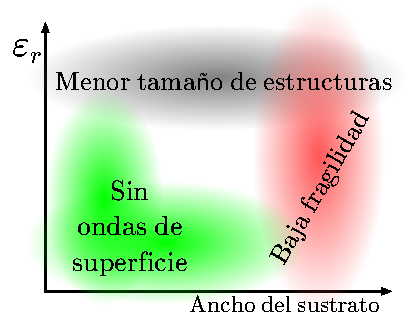
\includegraphics[width=1\textwidth]{Presentacion/problema_microstrip.pdf}
					\end{figure}
				
			\end{columns}
			\vspace{9pt}
			\centering {\footnotesize SW: Ondas de superficie. BW: Ancho de banda. $D$: Tamaño de la estructura. $h$: Ancho del sustrato.}
		\end{frame}
	
	
		\begin{frame}
			\frametitle{Modelo de líneas de transmisión}
			\centering Antena rectangular: Dos aperturas radiantes de ancho $W$ y altura $h$, sepadas una distancia $L$ por una línea de trasmisión de impedancia característica conocida $Z_0$.
			
			\begin{figure}[h]
				\centering
				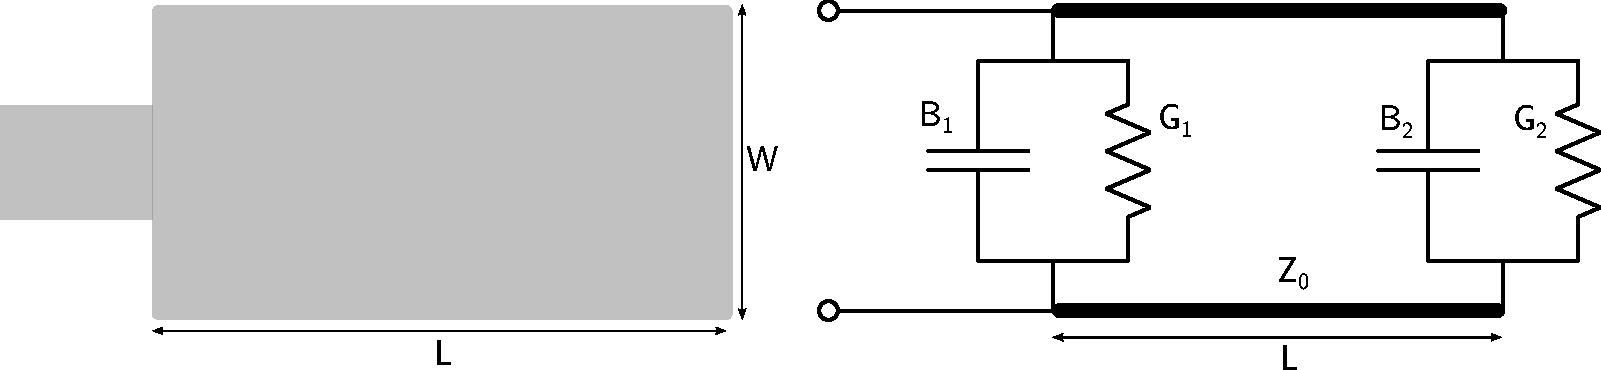
\includegraphics[width=0.9\textwidth]{intro_electro/circuito-equivalente-antena-ms.pdf}
			\end{figure}
		
			\textit{Fringing}: Considerado mediante el uso de una $L_{eff} = L + 2 \Delta L$.
		
		\end{frame}
	
		\begin{frame}
			\frametitle{Modelo de cavidades multimodo}
			\centering Antena rectangular: Cavidad cargada dieléctricamente, limitada por conductores eléctricos en sus caras superior e inferior, y por conductores magnéticos en sus caras laterales.
			
			\begin{align*}
				(f_r)_{nmp} = \frac{1}{2 \pi \sqrt{\mu \epsilon}} \sqrt{\left(\frac{m\pi}{h}\right)^2 + \left(\frac{n\pi}{L}\right)^2 + \left(\frac{p\pi}{W}\right)^2}
			\end{align*}
			
			\begin{figure}[h]
				\centering
				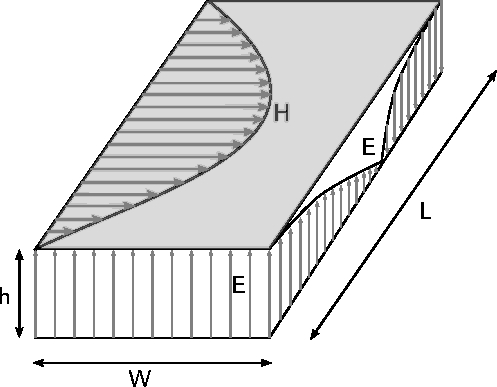
\includegraphics[width=0.49\textwidth]{intro_electro/distribucion-campos-microstrip.pdf}
			\end{figure}
		
		\end{frame}
	
		\begin{frame}
			\frametitle{Acoplamiento mutuo en antenas \textit{microstrip}}
					
			\begin{figure}[h]
				\centering
				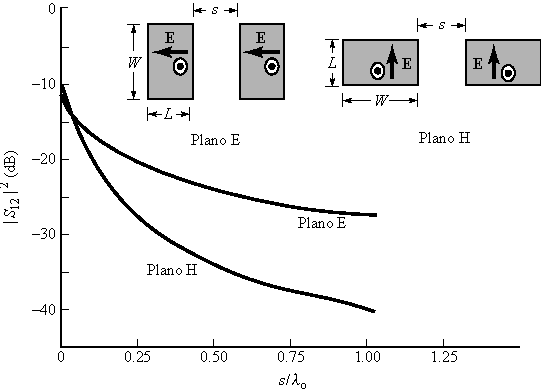
\includegraphics[width=0.9\textwidth]{intro_electro/pozar-acoplamiento.pdf}
			\end{figure}
		
		\end{frame}
		

%------------------------------------------------



\section{Fundamentos de EBGs}
	
	\begin{frame}
		\frametitle{Fundamentos básicos de EBGs}
		\tableofcontents[currentsection,hideothersubsections]
	\end{frame}

\subsection{Definiciones básicas}
	\begin{frame}
		\frametitle{Metamateriales y EBGs}
		\begin{columns}[c]
			\column{.51\textwidth}
			\begin{block}{Metamateriales}
				Estructuras artificiales \textbf{efectivamente homogéneas} para la longitud de onda de interés, que presentan \textbf{propiedades electromagnéticas que no se encuentran en la naturaleza}.
			\end{block}
		
			\begin{block}{EBGs, PBGs, cristales fotónicos}
				Estructuras articiales con capacidades para controlar (en general, atenuar) ondas electromagnéticas en un \textbf{rango de frecuencias} a partir de la \textbf{variación periódica} en el espacio de las propiedades del medio respecto de la propagación electromagnética.
			\end{block}
		
			\column{.46\textwidth}
			\begin{figure} [H]
				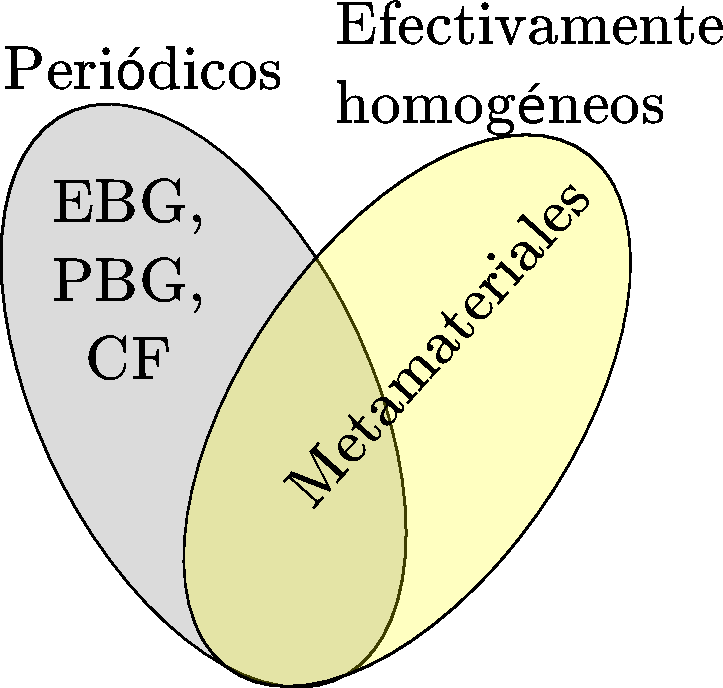
\includegraphics[width=0.9\textwidth]{Presentacion/ebg-metamateriales.pdf}
			\end{figure}
		\end{columns}
	\end{frame}
	
	\begin{frame}
		\frametitle{Reseña histórica}
		\only<1>{
			\begin{columns}[c]
				\column{0.55\textwidth}
				\begin{figure} [H]
					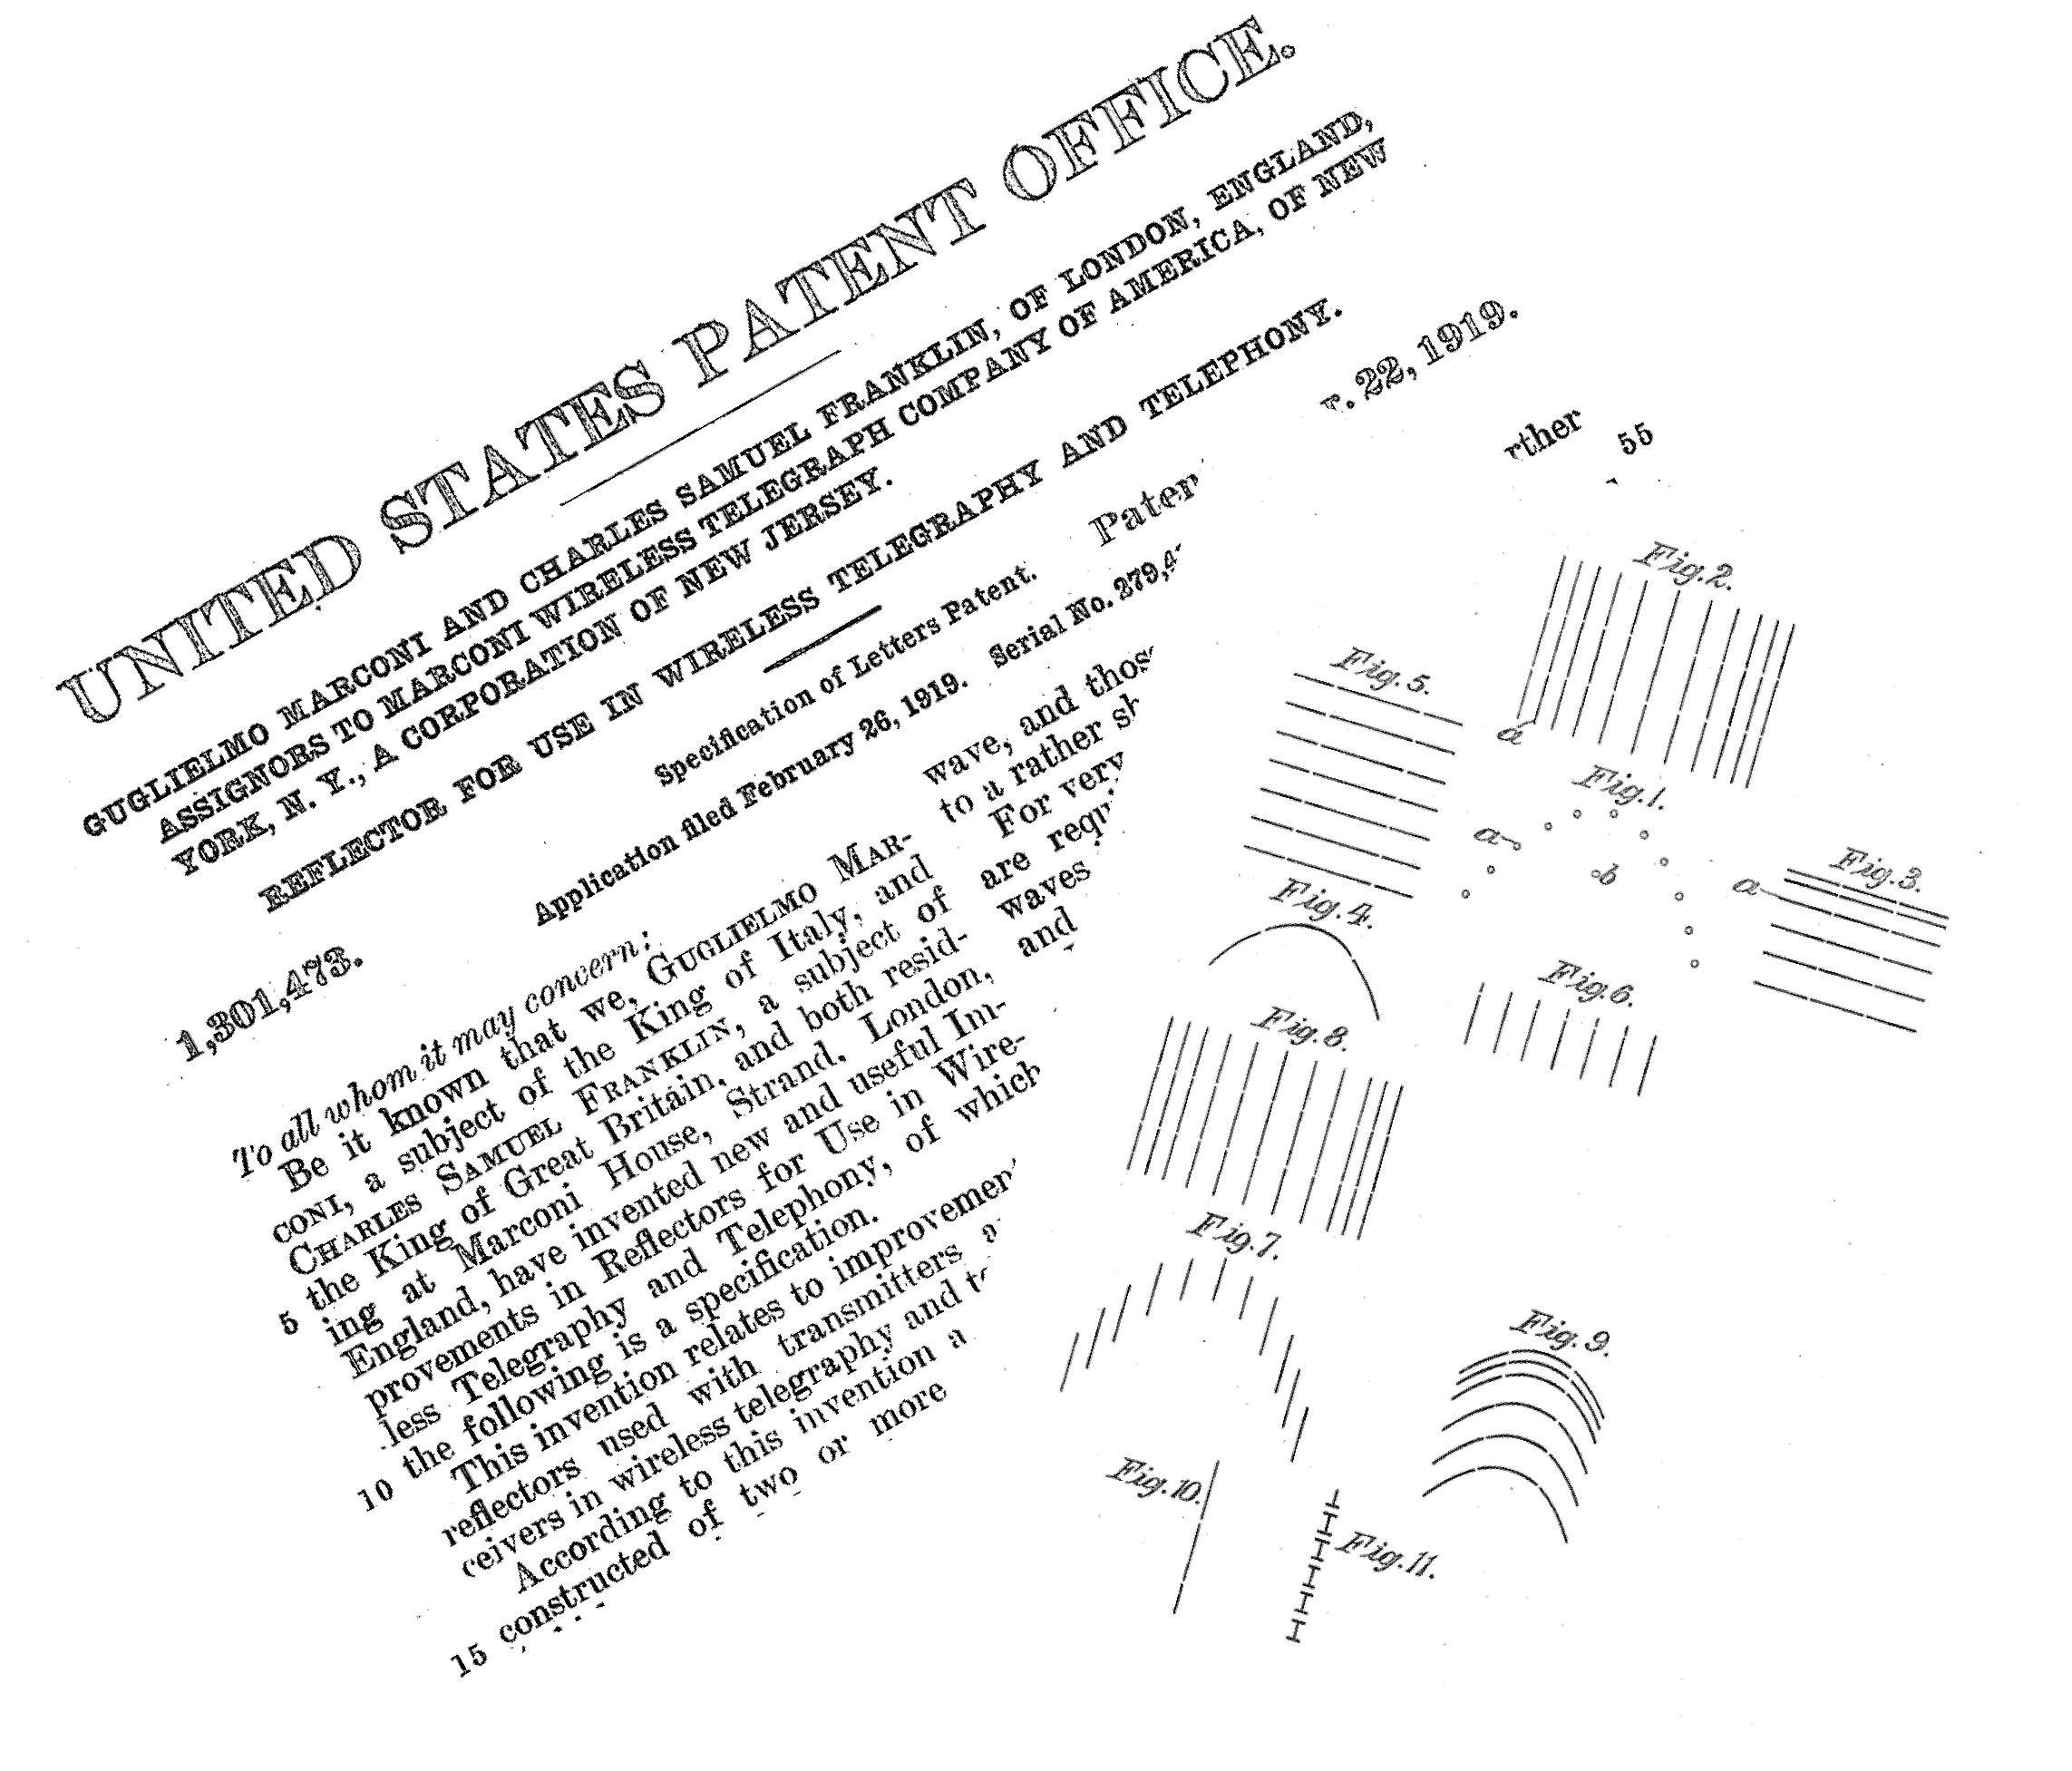
\includegraphics[width=1.2\textwidth]{Presentacion/patenteMarconi.pdf}
				\end{figure}
			
				\column{0.46\textwidth}
				\begin{itemize}
					\item Fines del siglo XVIII: \textbf{Rittenhouse} observó que algunos colores desaparecían cuando se veía luz a través de un pañuelo.
					\item 1919: Guglielmo \textbf{Marconi}, Charles Samuel \textbf{Franklin}: Conductores horizontales como superficie reflectiva para cierta frecuencia (¿Primer FSS?)
				\end{itemize}
			\end{columns}
		}
	
		
		\only<2>{
			\begin{itemize}
				\item 1946: Louis \textbf{Brillouin}: \textit{Wave propagacion in periodic structures: Electric filters and crystal lattices}. Restricciones a los vectores de onda $\gamma$ en un medio periódico.
				\item 1968: Viktor \textbf{Veselago}: Descripción teórica de LHS, velocidad de grupo antiparalela a la velocidad de fase.
			\end{itemize}
		
			\begin{figure}[h]
				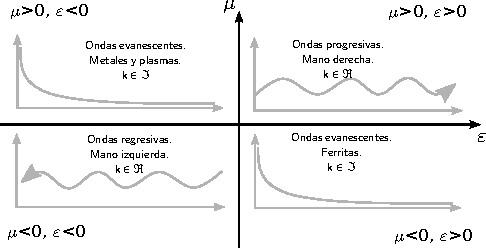
\includegraphics[width=0.8\textwidth]{Fundamentos/OndasSegunEyU.pdf}
			\end{figure}
		}
		
		\only<3>{
			\begin{figure}[htp]
				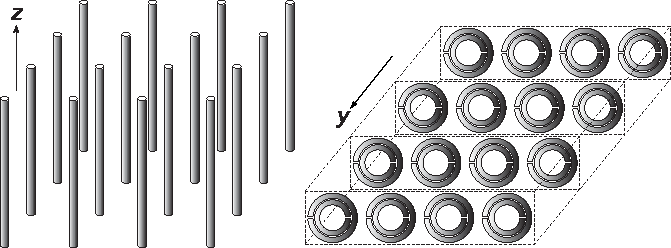
\includegraphics[width=0.8\textwidth]{Fundamentos/pendry.pdf}
			\end{figure}
			
			\begin{itemize}
				\item 1990: \textbf{Smith}: Split Ring Resonators en base a los trabajos de Pendry. Se construyó en 2000.
				\item 1990: \textbf{Ho, Chan, Soukulis}: Conjunto periódico de esferas dieléctricas. Banda prohibida.
				\item 1990: \textbf{Yablonovitch}. Estructura cristalina. Agujeros cilíndricos.
			\end{itemize}
		}
		
		\only<4>{
			\begin{figure}[htp]
				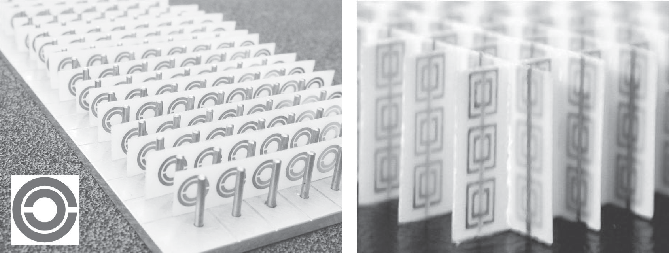
\includegraphics[width=\textwidth]{Fundamentos/metamateriales-smith.pdf}
			\end{figure}
		}
	

		\only<5>{
		\begin{itemize}
			\item 1999: \textbf{Sievenpiper}: HIS. Mushrooms. AMC + EBG.
			\item 2001: \textbf{Yang}: Uniplanar EBG (¿FSS o EBG?)
		\end{itemize}
		
		\begin{columns}[c]
			\column{.51\textwidth}
			\begin{figure}
				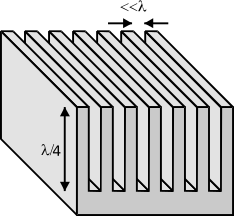
\includegraphics[width=0.8\textwidth]{Fundamentos/superficie-coarrugada.png}
			\end{figure}
		
			\column{.51\textwidth}
			\begin{figure}
				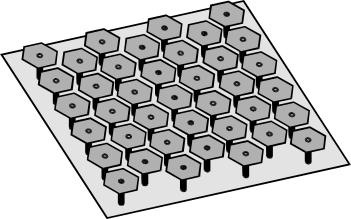
\includegraphics[width=\textwidth]{Fundamentos/sievenpiper.png}
			\end{figure}
		\end{columns}
		}
	\end{frame}
	
	\subsection{Bragg, Bloch-Floquet y espacio recíproco}
	
		\begin{frame}
			\frametitle{Difracción de Bragg}
		
			\centering 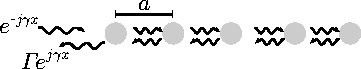
\includegraphics[width=0.6\textwidth]{Fundamentos/bragg1.pdf}
			
			\begin{align*}
			\Gamma_t = \Gamma e^{-j\gamma x} + \Gamma e^{-2j\gamma a} e^{-j\gamma x} + \Gamma e^{-4j\gamma a} e^{-j\gamma x} + ... = \Gamma e^{-j\gamma x} \frac{1}{1-e^{-2j\gamma a}}
			\end{align*}
			
			\centering Si $e^{-2j\gamma a} = 1$, la expresión diverge.
			
			 \begin{block}{\centering Condición de Bragg}
			 	\setlength\abovedisplayskip{0pt}
			 	\centering
			 		\begin{align*}
			 			\gamma = \frac{n\pi}{a}
			 		\end{align*}
			 \end{block}
		 
		 	\centering Y $\gamma$ está relacionado a la frecuencia, según el material.

			% Se podría dar la expresión más general en las diapositivas anexas.
		\end{frame}
		
		\begin{frame}
			\frametitle{Relación entre $\gamma$ y $\omega$ en el vacío: Diagrama de dispersión}
			
			\centering
			\setlength{\tabcolsep}{2em} % for the horizontal padding
			\renewcommand{\arraystretch}{2}% for the vertical padding
			\begin{tabular}{c|c}
				1D & 2D\\
				$\omega = c \beta$&$\omega = c \sqrt{\beta_x^2 + \beta_y^2}$\\
				&\\
				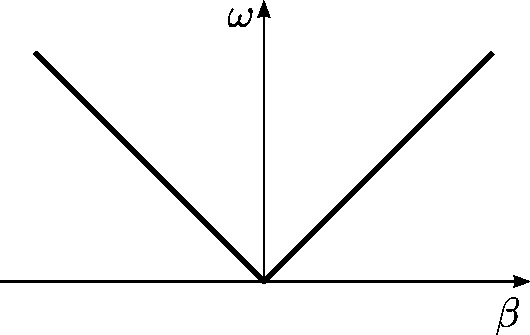
\includegraphics[width=0.4\textwidth]{Presentacion/dispersionvacio1d.pdf} & 	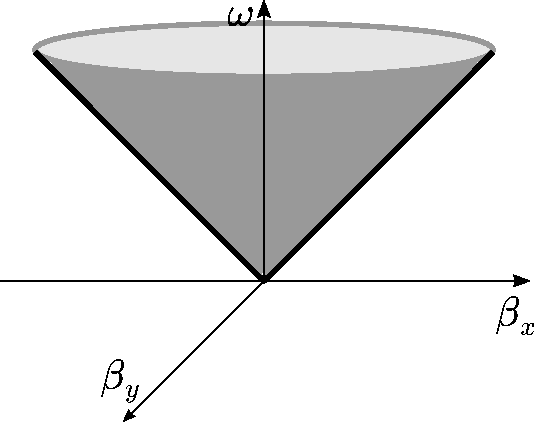
\includegraphics[width=0.3\textwidth]{Presentacion/dispersionvacio2d.pdf}\\	
			\end{tabular}
		
			
			\begin{block}{}
				Si hay números de onda prohibidos, ¿podría haber frecuencias prohibidas?
			\end{block}\textbf{}
		\end{frame}
		
		\begin{frame}
			\frametitle{Problema de autovalores}
			\centering Desacoplando las dos ecuaciones del rotor, se obtiene
			\begin{align*}
				\nabla \times \left(\frac{1}{\epsilon_r} \nabla \times \vec{H}(\vec{r}) \right) = \left(\frac{\omega}{c}\right)^2 \vec{H}(\vec{r}).
			\end{align*}
			
			\centering Se puede considerar un operador $\Theta$:
			
			\begin{block}{}
				\setlength\abovedisplayskip{0pt}
				\begin{align*}
					\hat{\Theta} = \nabla \times \frac{1}{\epsilon_r} \nabla \times
				\end{align*}
			\end{block}
			
			\centering De forma que
			
			\begin{block}{}
				\setlength\abovedisplayskip{0pt}
				\begin{align*}
					\hat{\Theta} \vec{H}(\vec{r}) = \left(  \frac{\omega}{c} \right)^2 \vec{H}(\vec{r})
				\end{align*}
			\end{block}
			
		\end{frame}
		
		\begin{frame}
			\frametitle{Problema de autovalores: Física cuántica}
			\renewcommand{\arraystretch}{2.5}% for the vertical padding
			\begin{tabular}{c c c}
				\toprule

				& \textbf{Cuántica} & \textbf{Electromagnetismo} \\ 
				\midrule
				Campo & $\Psi(\vec{r},t) = \Psi(\vec{r})e^{j\omega t}$ & $\vec{H}(\vec{r},t)=\vec{H}(\vec{r})e^{i\omega t}$ \\ 

				Problema de autovalores & $\hat{H}\Psi(\vec{r}) = E \Psi(\vec{r})$ & $\hat{\Theta} \vec{H}(\vec{r}) = \left(  \frac{\omega}{c} \right)^2 \vec{H}(\vec{r})$ \\ 

				Operador & $\hat{H} = \frac{-\hbar^2 \nabla^2}{2m} + V(\vec{r})$ &  $\hat{\Theta} = \nabla \times \frac{1}{\epsilon_r} \nabla \times$ \\ 

			\end{tabular}
			\vfill
			\centering Además, al igual que el Hamiltoniano, el operador $\Theta$ es hermítico.
						
		\end{frame}
		
\subsection{Teorema de Bloch-Floquet}
		\begin{frame}
		
		
			\only<1>{\frametitle{Teorema de Bloch-Floquet}
				\begin{columns}
					\column{.60\textwidth}
	
						\centering 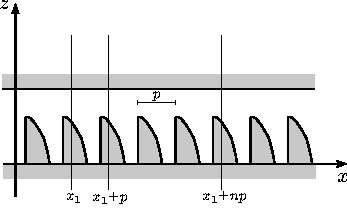
\includegraphics[width=1\textwidth]{Fundamentos/periodico-geometria.pdf}
	
				
					\column{.40\textwidth}
						\begin{block}{}
							\centering
							Gaston Floquet, 1883.
						\end{block}
					
						\begin{block}{}
							\centering
							\textbf{Teorema de Bloch}:
							
							Soluciones a la función de onda de un electrón en un cristal.
							\begin{align*}
								\phi(\vec{r}) = {\color{red}e^{j\vec{\gamma} \cdot \vec{r}}} u(\vec{r})
							\end{align*}
						\end{block}
			\end{columns}
			
			
			\begin{block}{}
				\setlength\abovedisplayskip{0pt}
				\begin{align*}
					E(x{\color{red}+d},y,z) = {\color{red}e^{-j \beta d}} E(x,y,z),
				\end{align*}
			\end{block}}
		
			\only<2>{\begin{center}
				\begin{figure}[y]
					\centering
					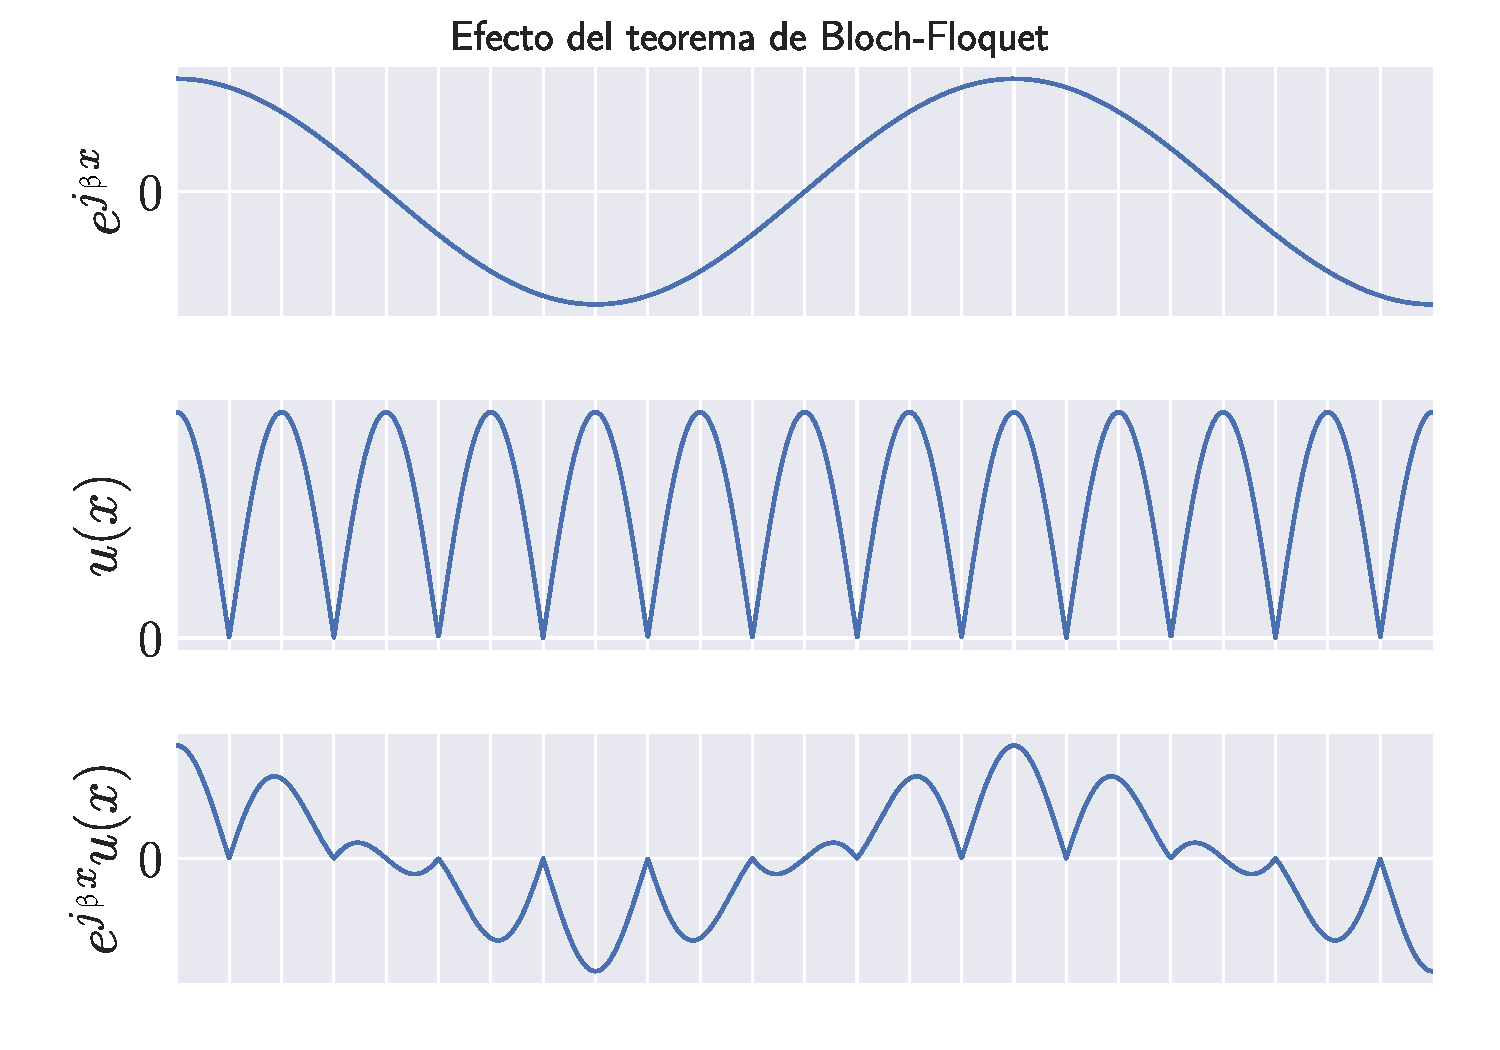
\includegraphics[width=0.75\textwidth]{Fundamentos/bloch.pdf}
				\end{figure}
			\end{center}
			\vspace{-20pt}
			\begin{center}
				\begin{figure}[h]
					\centering
					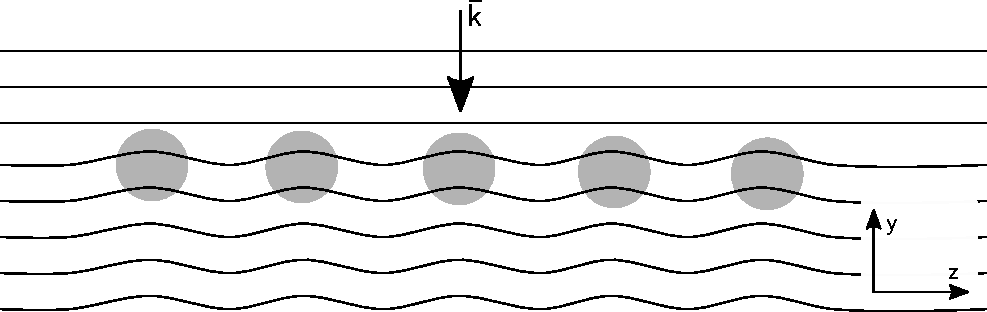
\includegraphics[width=0.6\textwidth]{Fundamentos/bloch-ortogonal.pdf}
				\end{figure}
			\end{center}
		}
		\only<3>{
			\begin{columns}[c]
				\column{.65\textwidth}
				\begin{figure}[h]
					\centering
					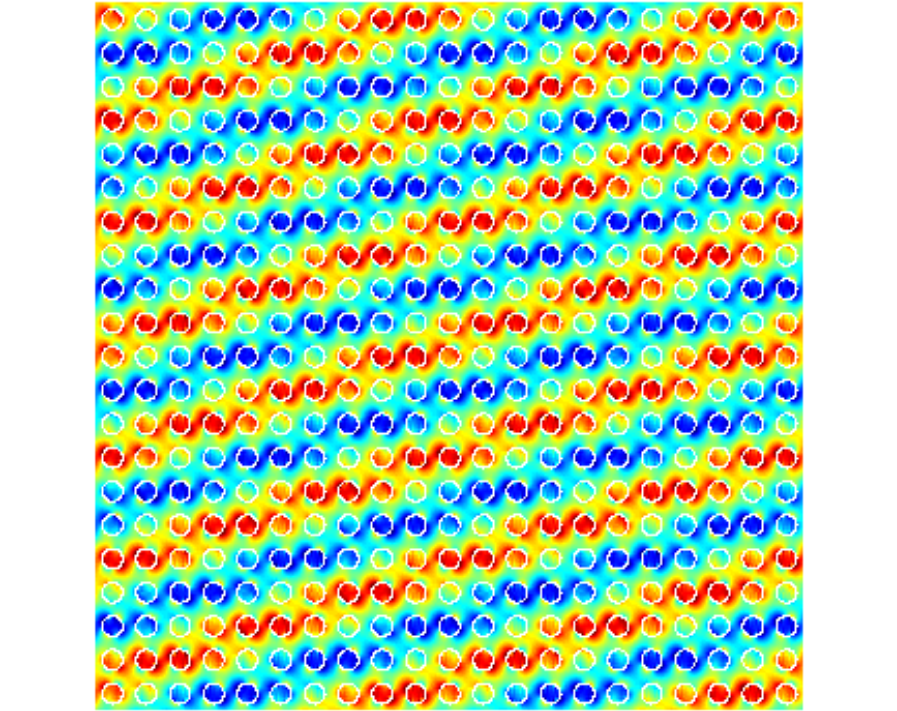
\includegraphics[width=\textwidth]{Presentacion/bloch-2d-1.png}
				\end{figure}
				
				\column{.35\textwidth}
				\begin{figure}[h]
					\centering
					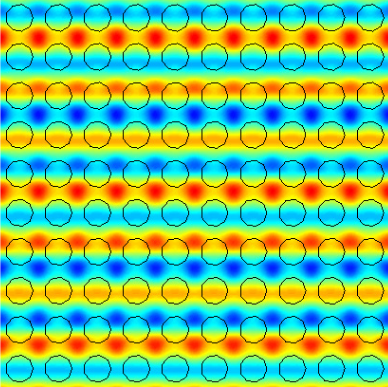
\includegraphics[width=0.9\textwidth]{Presentacion/bloch-2d-2.png}
				\end{figure}
				\vspace{-10pt}
				\begin{figure}[h]
					\centering
					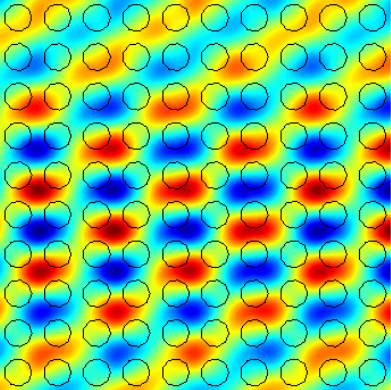
\includegraphics[width=0.9\textwidth]{Presentacion/bloch-2d-3.png}
				\end{figure}
				
			\end{columns}
			
		}	
		\end{frame}

\subsection{Diagrama de dispersión de una estructura periódica}
		\begin{frame}
			\frametitle{Armónicos espaciales y Celda de Brillouin}
			\only<1>{
				\centering Para una periodicidad en una dirección ($x$) en que el espacio tiene comportamiento periódico, se puede desarrollar la Transformada de Fourier:
				
				\begin{align*}
					F(x,y,z) = \sum_{n=-\infty}^{\infty} F_{n}(y,z) e^{-j n \frac{2\pi}{p} x}
				\end{align*}
				
				\centering Tras aplicar las condiciones de Bloch:
				\begin{columns}[c]
					\column{.55\textwidth}
					\begin{block}{}
						\setlength\abovedisplayskip{0pt}
						\begin{gather*}
							 E(x,y,z,t) = e^{j\omega t} \sum_{n=-\infty}^{\infty} E_n(y,z) e^{-j{\color{red}\gamma_n} x},\\
							 \gamma_n = \gamma_0 + n \frac{2\pi}{p}.
						\end{gather*}
					\end{block}
					
					\column{.4\textwidth}
					
					\begin{block}{}
						\centering Campo en un medio periódico:
						
						Suma de \textbf{infinitas armónicas}.
					\end{block}
					
				\end{columns}
			\vfill
			Cada término: armónica espacial asociada a un $\gamma_n$.
		}
		\only<2>{
			\begin{block}{}
				\setlength\abovedisplayskip{0pt}
				\begin{align*}
					\gamma_n = \gamma_0 + n \frac{2\pi}{p}
				\end{align*}
			\end{block}
		
			\centering La \textbf{velocidad de fase} es distinta para cada modo.
			
			\begin{block}{}
				\setlength\abovedisplayskip{0pt}
				\begin{align*}
					v_p^n = \frac{\omega}{\beta_n} = \frac{\omega}{\beta_0 + 2\pi n/p}
				\end{align*}
			\end{block}
			
			\centering La \textbf{velocidad de grupo} es la misma para todas las armónicas.
			
			\begin{block}{}
				\setlength\abovedisplayskip{0pt}
				\begin{align*}
					v_g^n = \frac{d\omega}{d\beta_n} = \frac{d\omega}{d(\beta_0 +2\pi n/p)} = \frac{d\omega}{d\beta_0} = v_g^0.
				\end{align*}
			\end{block}
			\begin{figure}[h]
				\centering
				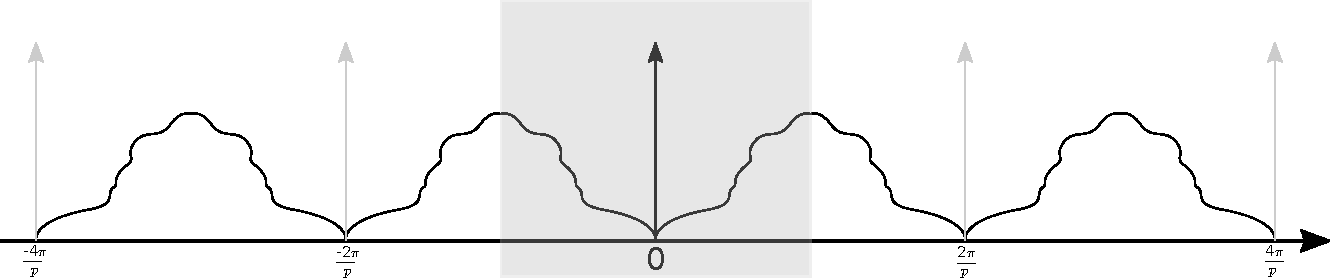
\includegraphics[width=0.75\textwidth]{Presentacion/brillioun-1d.pdf}
			\end{figure}
		}
	
		\centering
		\includegraphics<3,4,5>[width=0.9\textwidth]{Presentacion/dispersion-ejemplo-1.pdf}%
		\only<3,4,5>{\vfill}
			
		\centering
		\includegraphics<4>[width=0.9\textwidth]{Presentacion/dispersion-ejemplo-2.pdf}%

		\centering
		\includegraphics<5>[width=0.9\textwidth]{Presentacion/dispersion-ejemplo-3.pdf}%

		\centering
		\includegraphics<6,7>[width=0.9\textwidth]{Presentacion/dispersion-ejemplo-4.pdf}%
		\vfill

		\only<7>{
			\centering \textbf{Principio variacional: Los estados de menor energía la concentran en la zona de mayor $\epsilon_r$.}}
			
		\centering \includegraphics<7>[width=0.9\textwidth]{Presentacion/dispersion-ejemplo-5.pdf}%
		\only<7>{
				
			\small{Debido a la ortogonalidad de los autoestados asociados al operador, existen estados, de mayor energía, donde la misma se concentra en el menor $\epsilon_r$ para el mismo $\beta$.}
		}
		
	
	
		\end{frame}

\subsection{Red de Bravais y red recíproca}
		% Aca va lo del ppio variacional
	
		\begin{frame}
		\frametitle{Red de Bravais y Celda de Wigner-Seitz}
			\begin{columns}[c]
				\column{.55\textwidth}
				\begin{figure}[h]
					\centering
					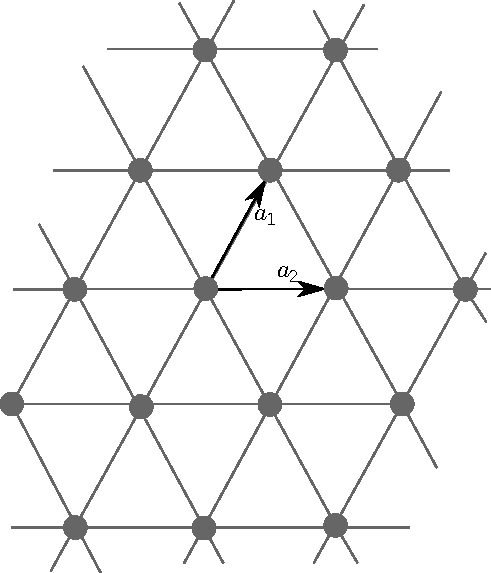
\includegraphics[width=0.9\textwidth]{Fundamentos/direct-and-reciprocal-triangle-lattice.pdf}
				\end{figure}
				\column{.55\textwidth}
				\begin{figure}[h]
					\centering
					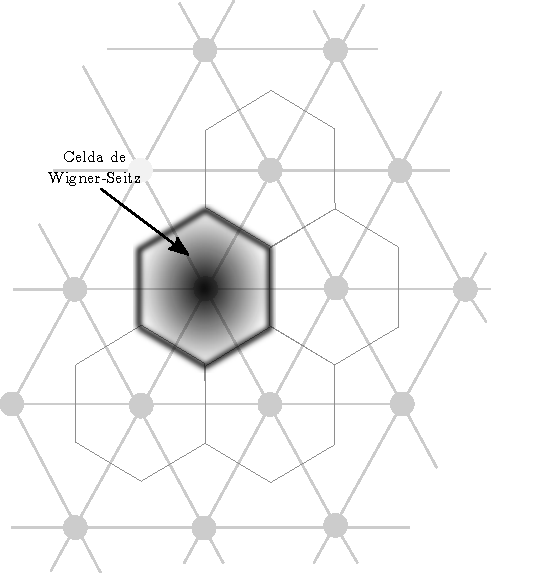
\includegraphics[width=0.9\textwidth]{Fundamentos/direct-and-reciprocal-triangle-lattice-zoom2.pdf}
				\end{figure}
			\end{columns}
		\end{frame}
	
		\begin{frame}
			\frametitle{Red recíproca y Celda de Brillouin}
			\begin{columns}[c]
				\column{.55\textwidth}
				\begin{figure}[h]
					\centering
					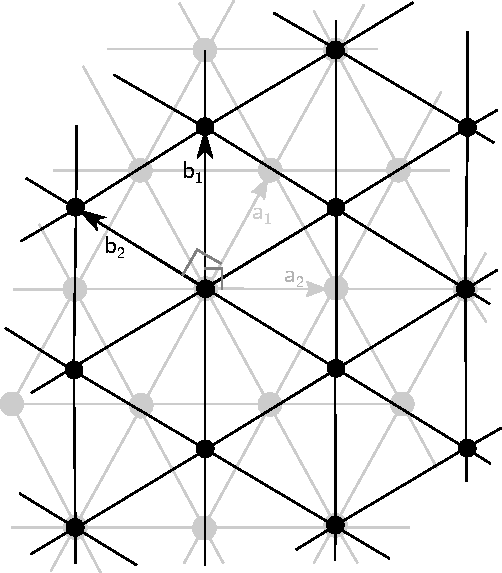
\includegraphics[width=0.9\textwidth]{Fundamentos/direct-and-reciprocal-triangle-lattice-zoom4.pdf}
				\end{figure}
				\column{.55\textwidth}
				\begin{figure}[h]
					\centering
					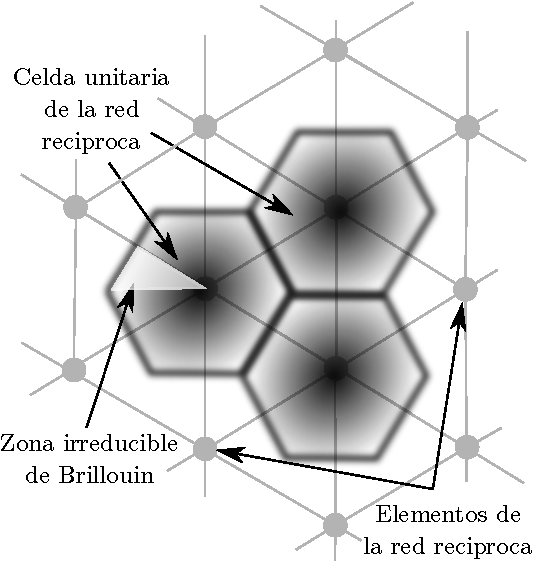
\includegraphics[width=0.8\textwidth]{Fundamentos/direct-and-reciprocal-triangle-lattice-zoom5.pdf}
				\end{figure}
			\end{columns}
		\end{frame}
	
		\begin{frame}
			\frametitle{Red de Bravais y red recíproca para celdas rectangulares}
				\begin{figure}[h]
					\centering
					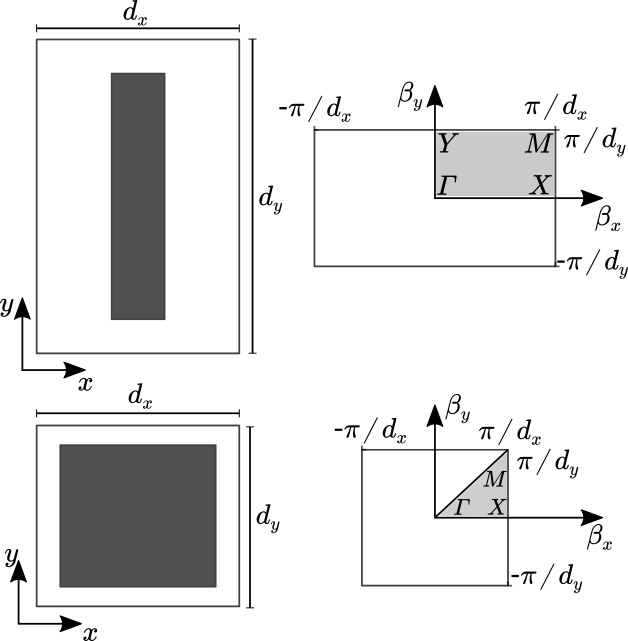
\includegraphics[width=0.6\textwidth]{Fundamentos/rectangulo-cuadradado.pdf}
				\end{figure}
		\end{frame}
		
		\begin{frame}
			\only<1>{\begin{figure}[h]
					\centering
					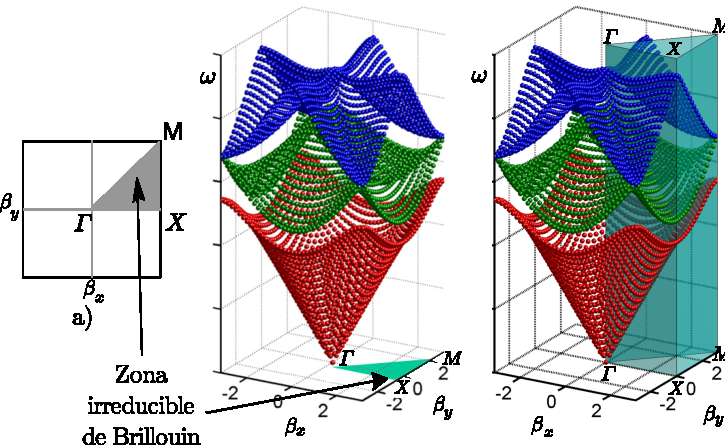
\includegraphics[width=0.8\textwidth]{Presentacion/diagrama-dispersion-deduccion-1.pdf}
				\end{figure}}
			\only<2>{
					\begin{figure}[h]
						\centering
						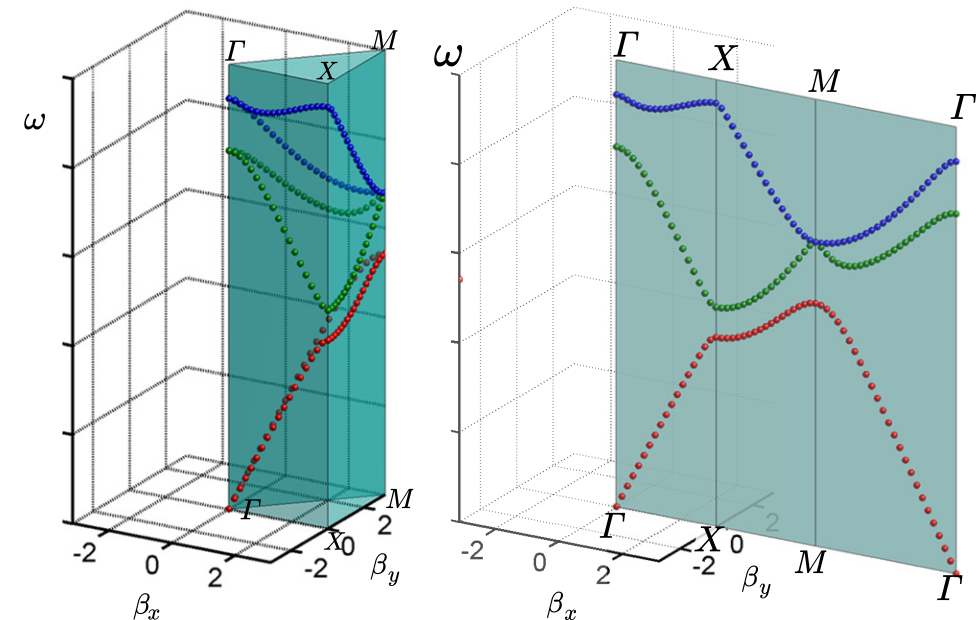
\includegraphics[width=0.8\textwidth]{Presentacion/diagrama-dispersion-deduccion-2.png}
				\end{figure}}
			\only<3>{
					\begin{figure}[h]
						\centering
						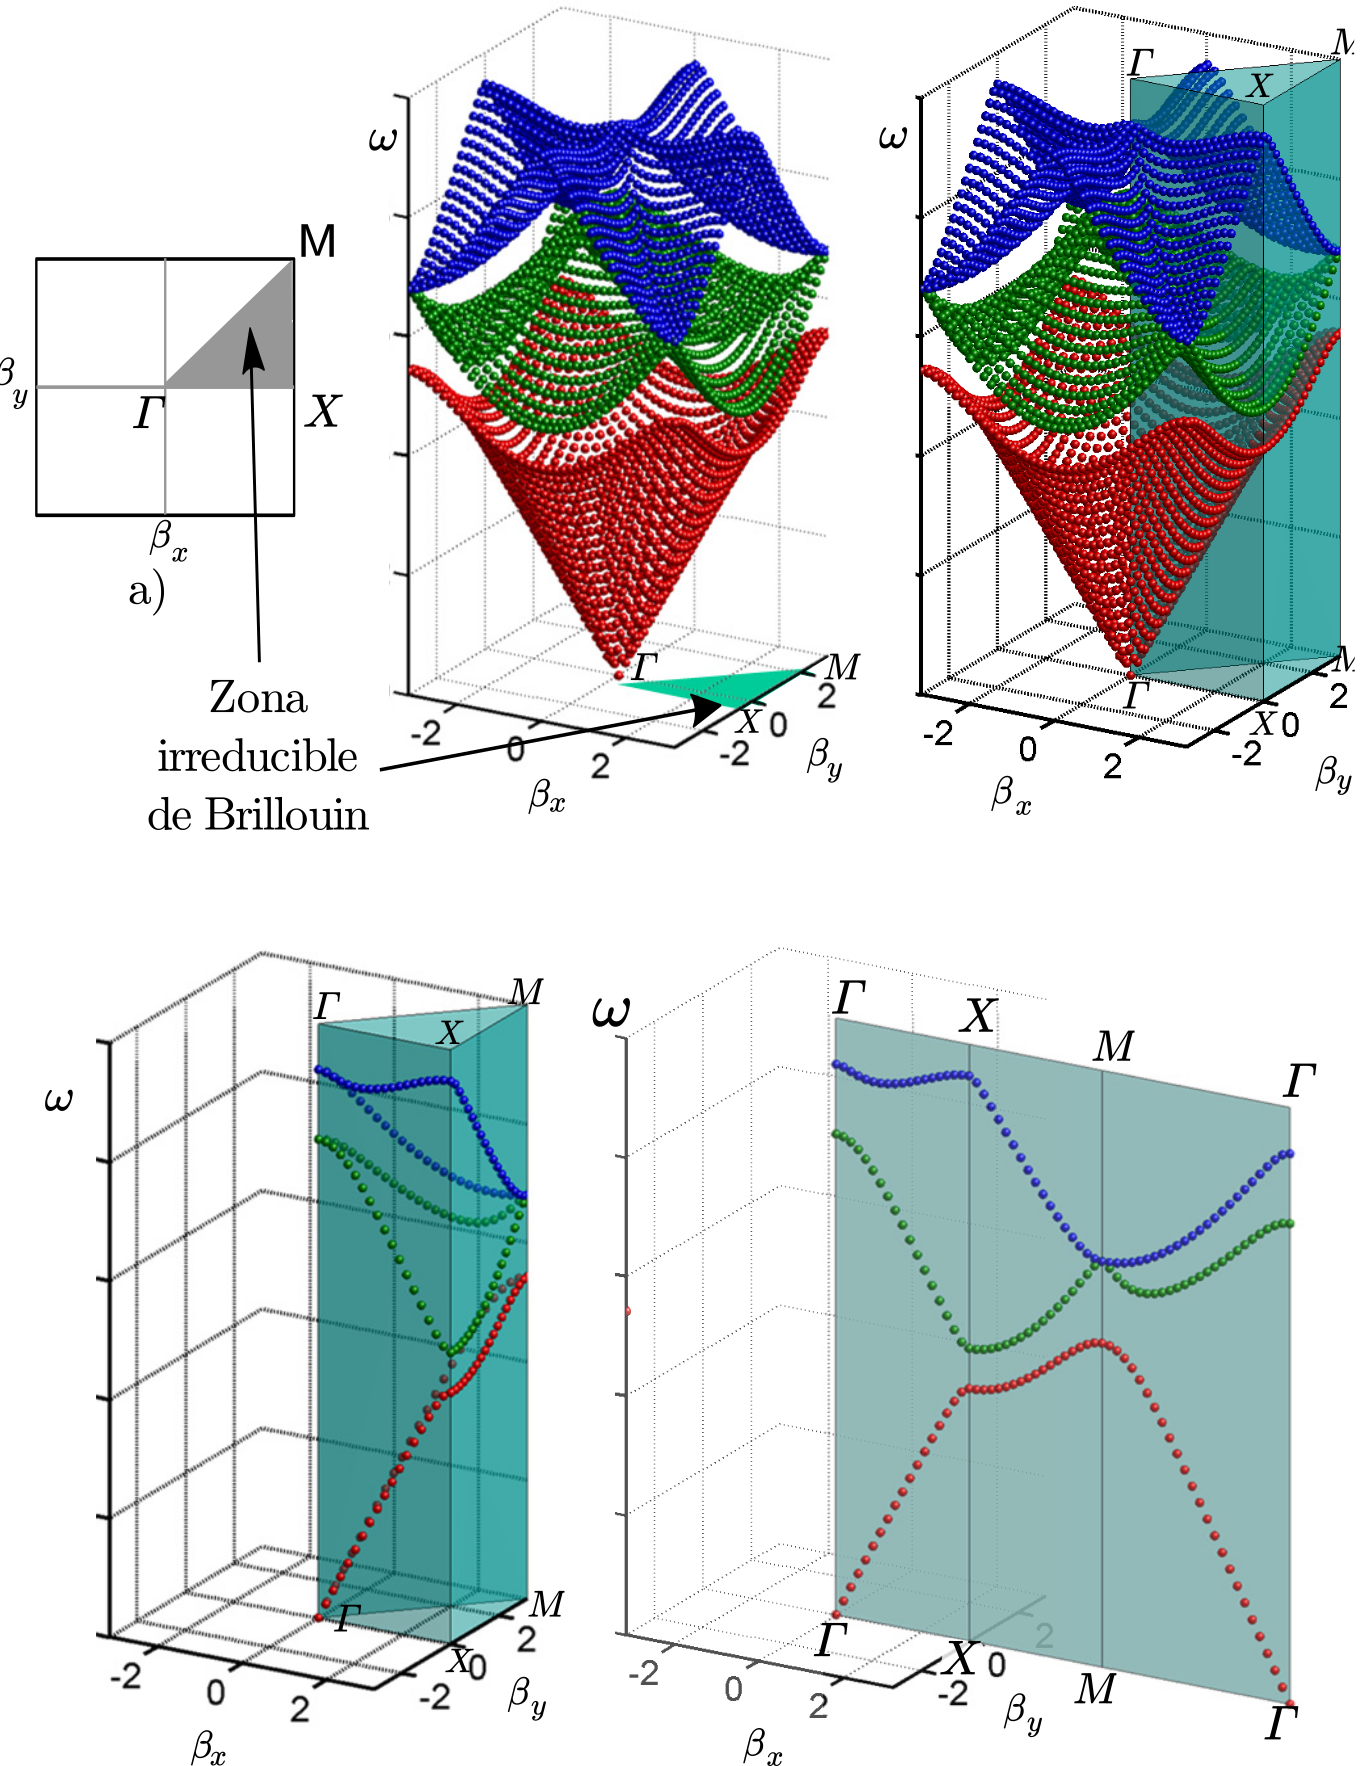
\includegraphics[width=0.55\textwidth]{Presentacion/diagrama-dispersion-deduccion.png}
				\end{figure}}
			\only<4>{
				\centering 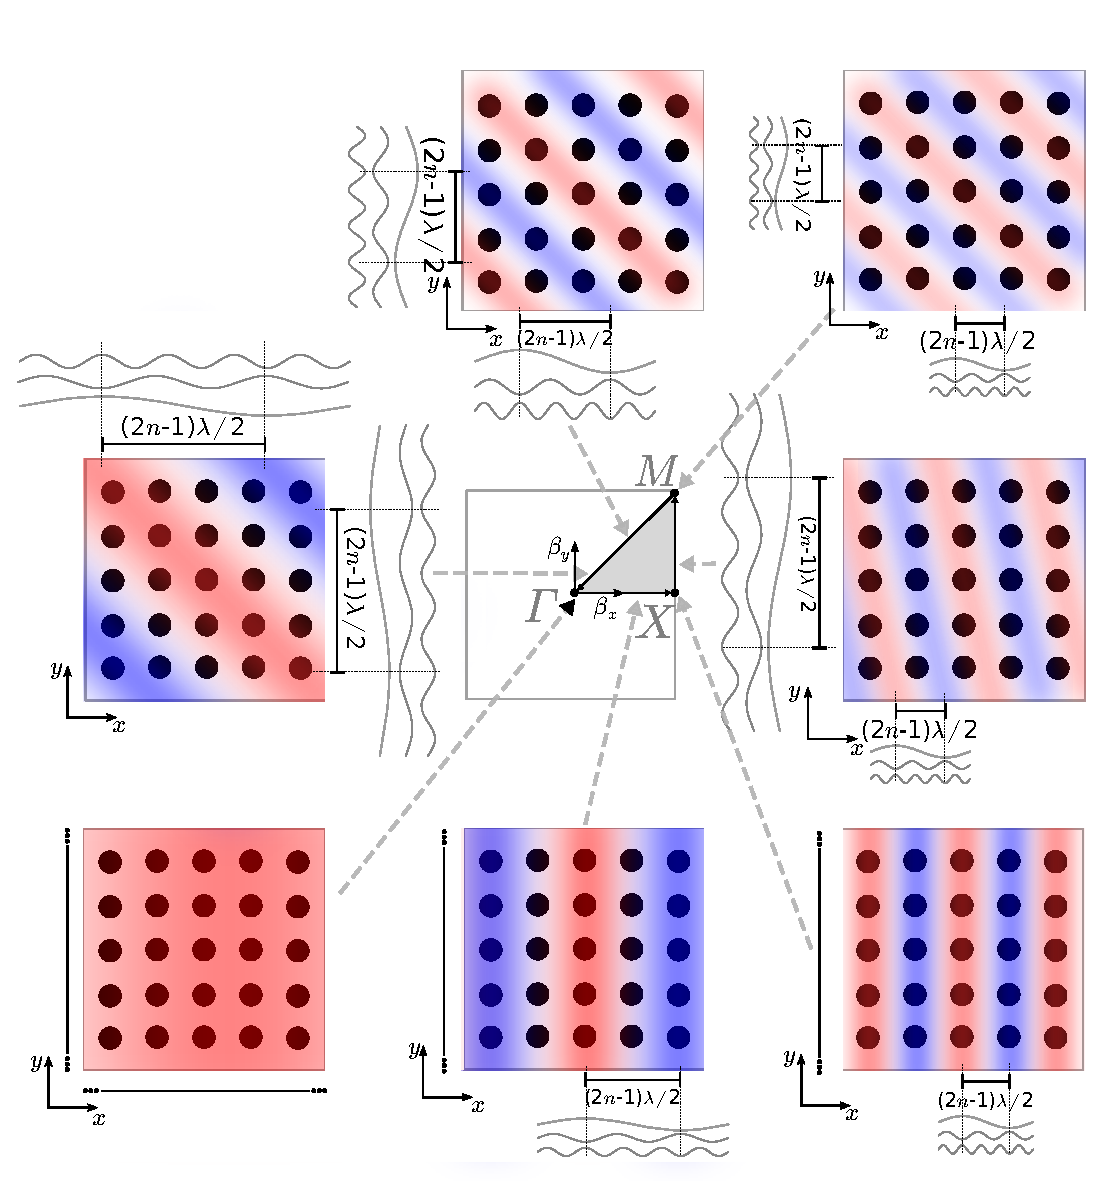
\includegraphics[width=0.67\textwidth]{Fundamentos/Fisica-DiagramaDeFase.pdf}
			}
		\end{frame}
		
		\begin{frame}
		\frametitle{Diagrama de dispersión bidimensional en medio homogéneo}
			\begin{columns}[c]
				\column{0.5\textwidth}
				\begin{figure}[h]
					\centering
					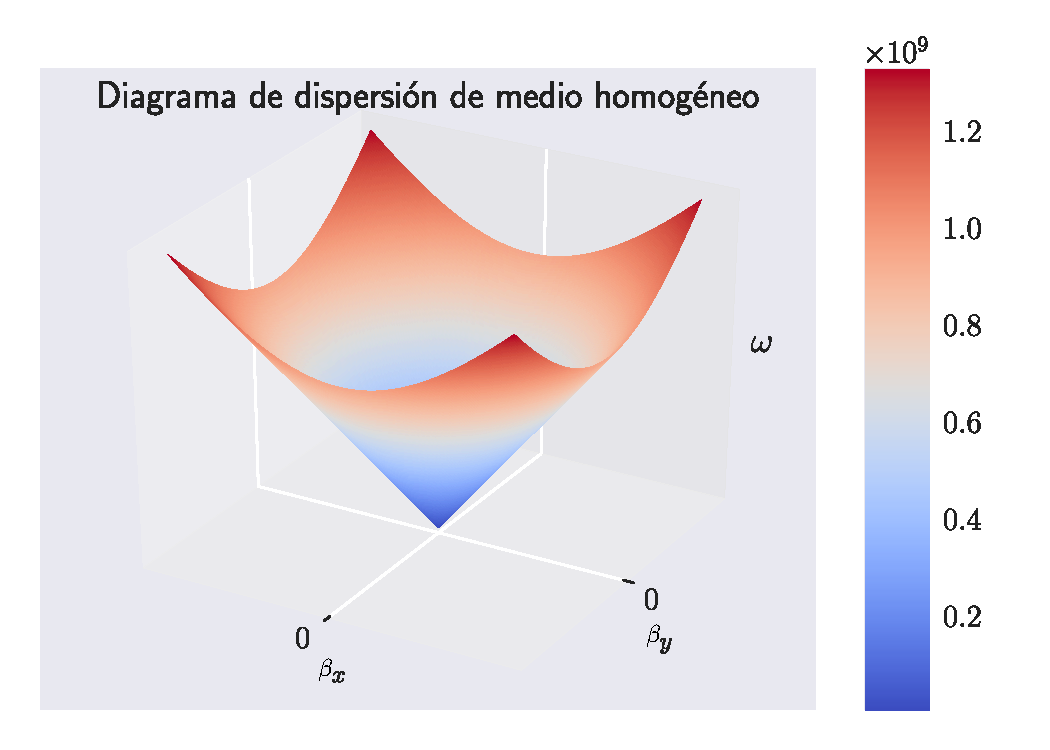
\includegraphics[width=\textwidth]{Fundamentos/plot-cono-luz.pdf}
				\end{figure}
				\column{0.55\textwidth}
				\begin{figure}[h]
					\centering
					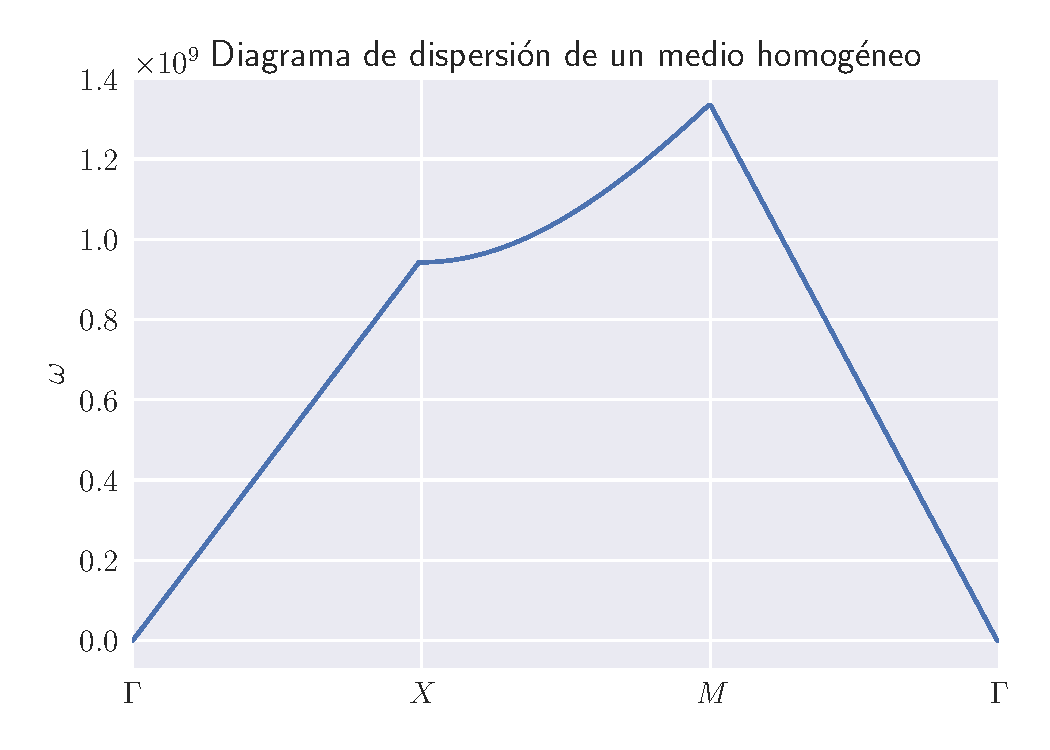
\includegraphics[width=\textwidth]{Fundamentos/diag-dispersion-vacio-2d.pdf}
				\end{figure}
			\end{columns}
		\end{frame}

\section{Modelado numérico de estructuras EBG}

		\begin{frame}
			\frametitle{Modelado numérico de estructuras EBG}
			\tableofcontents[currentsection,hideothersubsections]
		\end{frame}

		\begin{frame}
			\frametitle{Modelado de estructuras EBG}
			
			\only<1>{\renewcommand{\arraystretch}{2}% for the vertical padding
			\begin{tabular}{>{\centering\bfseries}m{0.8in} >{\centering}m{0.2in} >{\centering}m{2in} >{\centering\arraybackslash}m{1in}}
				\toprule
				\textbf{Método} & \centering\textbf{Dom} & \centering \textbf{Tipo de problema} & \textbf{Software}\\
				\midrule
				FEM & \centering f & \centering Pequeños y complejos (incógnitas $\propto$ volumen). & \textit{HFSS} \\
				FDTD & \centering t & \centering Banda ancha. Resonantes (autovalores). & \textit{CST}\\
				MOM & \centering f & \centering Recintos abiertos. & \textit{NEC-2, ADS, FEKO}\\
				\bottomrule
			\end{tabular}}
			
			\only<2>{
				Métodos semianalíticos:
			\begin{itemize}
				\item \textbf{TMM}: Método de matrices de transmisión (2D).
				\item {\color{red}\textbf{TLM}: Método de matrices de líneas de transmisión (2D, 3D).}
				\item {\color{red}\textbf{Circuitos equivalentes} (primer modo, bajas frecuencias, 2D).}
			\end{itemize}
		\vfill
		\centering El modelo de circuitos equivalentes no es capaz, por sí mismo, de predecir diagramas de dispersión.}
		\end{frame}
	
		\begin{frame}
			\frametitle{Problema de autovalores con métodos de onda completa}
			\begin{columns}[c]
				\column{0.55\textwidth}
					\centering 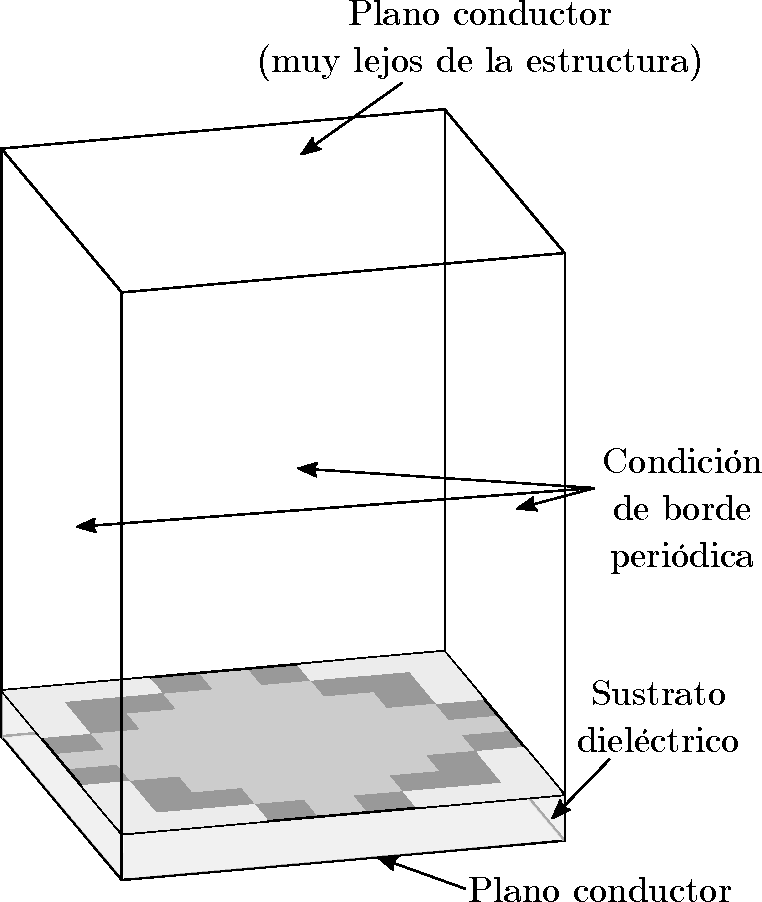
\includegraphics[width=0.95\textwidth]{Modelado/esquema-simulacion-periodica.pdf}
				\column{0.40\textwidth}
					\begin{block}{}
						\centering Simulación de una única celda unitaria describe la estructura infinita.
					\end{block}
				
					\begin{block}{\centering PBC}
						\centering Bloch: Campo periódico con igual periodicidad que el material, a excepción de un factor de fase.
						\vspace{0.6cm}
											
						\textbf{Condición de borde: Diferencia de fase entre paredes enfrentadas}.
					\end{block}
			\end{columns}

		\end{frame}
\subsection{Parches unidos por trazas \textit{microstrip}}

		\begin{frame}
			\only<1>{\frametitle{Parches cuadrados unidos por trazas \textit{microstrip}}
				\begin{figure}[h]
					\centering
					\includegraphics[width=0.5\textwidth]{Modelado/orlandi-celda.pdf}
				\end{figure}
				\begin{block}{}
					\centering Zona de Brillouin triangular.
				\end{block}}
			\only<2>{
				\begin{figure}[h]
					\centering
					\includegraphics[width=1\textwidth]{Modelado/orlandi-modo1-Enorma-Etangencial.pdf}
				\end{figure}
			}
		
			\only<3>{
				
				\begin{figure}[h]
					\centering
					\includegraphics[width=1\textwidth]{Modelado/orlandi-modo1-EH-fases.pdf}
				\end{figure}
			}
		
			\only<2,3>{
				\begin{figure}[h]
					\centering
					\includegraphics[width=0.55\textwidth]{Presentacion/modos-de-propagacion-ilustracion.pdf}
				\end{figure}
			}

		\end{frame}
		
		\begin{frame}
		\only<1>{

				\frametitle{Diagrama de dispersión por método de onda completa}
				\begin{figure}[h]
					\centering
					\includegraphics[width=\textwidth]{Presentacion/diagdisp-1.pdf}
				\end{figure}
		}
	
		\only<2>{
			\frametitle{Diagrama de dispersión por método de onda completa}
			\begin{figure}[h]
				\centering
				\includegraphics[width=\textwidth]{Presentacion/diagdisp-2.pdf}
			\end{figure}
		}
	
		\only<3>{
			\frametitle{Diagrama de dispersión por método de onda completa}
			\begin{figure}[h]
				\centering
				\includegraphics[width=\textwidth]{Presentacion/diagdisp-3.pdf}
			\end{figure}
			\centering Línea de vista: Comportamiento de onda plana que circula por un medio homogéneo de ese material.
		}
	
		\only<4>{
			\frametitle{Diagrama de dispersión por método de onda completa}
			\begin{figure}[h]
				\centering
				\includegraphics[width=\textwidth]{Presentacion/diagdisp-4.pdf}
			\end{figure}
		\centering \textit{Bandgaps}: Se calculan para las tres direcciones en forma separada, por debajo de la línea de vista del vacío.
		}
		\end{frame}
	
		\begin{frame}
			\frametitle{Análisis paramétrico de la celda}
				\only<1>{\framesubtitle{Variación del ancho del puente}
					\includegraphics[width=\textwidth]{Modelado/Orlandi-DeltaAnchoConector-comparacion.pdf}
				}
				\only<2>{\framesubtitle{Variación del largo del puente}
					\includegraphics[width=\textwidth]{Modelado/Orlandi-DeltaSeparacionParches-DeltaTamanioCelda-ParcheFijo-Comparacion.pdf}
				}
				\only<3>{\framesubtitle{Variación del tamaño de celda}
					\includegraphics[width=\textwidth]{Modelado/Orlandi-DeltaTamanioCelda-RelacionParcheFija-Comparacion.pdf}
				}
				\only<4>{\framesubtitle{Variación del ancho del sustrato}
					\centering \includegraphics[width=0.94\textwidth]{Modelado/Orlandi-3direcciones-anchoSustrato-Comparacion.pdf}
				}
			
		\end{frame}

\subsection{Celda de Yang: Modelo circuital}
		\begin{frame}
			\frametitle{Celda de Yang, Ma, Qian e Itoh}
				\begin{columns}[c]
					\column{0.5\textwidth}
					\centering \includegraphics[width=\textwidth]{Modelado/yang-celda.pdf}
					\column{0.5\textwidth}
					\centering \includegraphics[width=\textwidth]{Presentacion/yang-modo1-Enorma-Etangencial.pdf} 
				\end{columns}
		\end{frame}
	
		\begin{frame}
			\frametitle{Modelo circuital I}
			\only<1>{
				\centering No se tendrán en cuenta efectos de alta frecuencia.\\
				\vspace{0.3cm}
				\centering \includegraphics[width=0.8\textwidth]{Fundamentos/circuito-equivalente-celda-YANG-2.pdf}
				\vspace{.5cm}
				
				\centering
				\begin{tabular}{c c c c c c c }
					\toprule
					$d$ & $l$ & $w$ & $d_l$ & $g$ & $h$ & $d_w$\\ 
					\midrule
					$22.6\;mm$ & $6\;mm$ & $1.1\;mm$ & $0.8\;mm$ & $0.8\;mm$ & $1.6\;mm$ & $16.6\;mm$\\ 
				\end{tabular}
			
			
				\begin{textblock*}{20mm}(105mm,20mm)
					\begin{block}{}
						\centering $f_r = \frac{1}{2\pi\sqrt{LC}}$
					\end{block}
				\end{textblock*}
			
				\begin{textblock*}{20mm}(105mm,45mm)
					\begin{block}{}
						\centering Filtro \textit{notch}.
					\end{block}
				\end{textblock*}
		}
		\only<2>{
			\framesubtitle{Inductancia de puente, $L_b$}
			\centering Tres acercamientos distintos:
			\begin{itemize}
				\item Kim, Schutt-Ainé (2008)): 
					\begin{align*}
						L_{b} = 0.2\; \text{nH/mm} \cdot \ln \left(2\pi \frac{h}{w}\right)
					\end{align*}
				\item C. Paul (2010):
					\begin{align*}
						L_{b} = \begin{cases}
						\frac{60 l}{c} \ln \left( \frac{8h}{w} + \frac{w}{4h} \right) \text{ para } \frac{w}{h}\leq 1\\
						\frac{120 \pi l}{c} \frac{1}{w/h+1.393+0.667\ln(w/h+1.444)} \text{ para } \frac{w}{h} > 1 \\
						\end{cases}
					\end{align*}
				\item Ansys Q3D Extractor, usando BEM (\textit{Boundary Element Method}).
			\end{itemize}
			\vfill
			
			\centering
			\begin{tabular}{ c c c }
				\toprule
				Kim, Shutt-Ainé & C. Paul & \textit{Ansys Q3D Extractor}\\ 
				\midrule
				$7.34\;nH$ & $8.2\;nH$ & $7.7\;nH$\\ 
				\hline 
			\end{tabular}
		}
	
		\only<3>{
			\framesubtitle{Capacidad entre celdas vecinas, $C_g$, y con plano de tierra, $C_p$}
			\centering Dos acercamientos distintos:
			\begin{columns}[c]
				\column{0.5\textwidth}
					\begin{itemize}
						\item C. Paul (2010): 
						\begin{align*}
						C_{g} = \frac{d_w\epsilon_0(1+\epsilon_r)}{\pi}\cosh^{-1}\left(\frac{2 d_w + g}{g}\right)
						\end{align*}
						\item \textit{Ansys Q3D Extractor}.
					\end{itemize}
				
					\centering
					\begin{tabular}{c c}
						\toprule
						C. Paul & \textit{Ansys Q3D Extractor} \\ 
						\midrule 
						$475\; fF$ & $130\; fF$\\ 
					\end{tabular}
				\column{0.5\textwidth}
					\centering \includegraphics[width=0.8\textwidth]{Modelado/capacidad-cg-Q3D.png}
			\end{columns}
		
			\noindent\makebox[\linewidth]{\rule{\paperwidth}{0.4pt}}
		
			\begin{columns}[c]
				\column{0.5\textwidth}
					\begin{itemize}
						\item Placas planas paralelas: 
						\begin{align*}
						C_{p} = A \frac{\epsilon_0\epsilon_r}{h}
						\end{align*}
						\item \textit{Ansys Q3D Extractor}.
					\end{itemize}
				\column{0.55\textwidth}
					\centering
					\begin{tabular}{c c}
						\toprule
						Placas planas & \textit{Ansys Q3D Extractor} \\ 
						\midrule 
						$11.14\;pF$ & $12.26\; pF$\\ 
					\end{tabular}
			\end{columns}
		}
	
		\only<4>{
			\framesubtitle{Resultado de la simulación}
			
			\centering \includegraphics[width=0.9\textwidth]{Modelado/3-4.pdf}
			
			\begin{textblock*}{20mm}(25mm,55mm)
				\begin{block}{}
					\centering $f_r$ no coincide.
				\end{block}
			\end{textblock*}
			
			\begin{textblock*}{30mm}(95mm,39mm)
				\begin{block}{}
					\centering Comportamiento a altas frecuencias.
				\end{block}
			\end{textblock*}
		}
		\end{frame}
	
		\begin{frame}
			\frametitle{Modelo circuital II}
			\only<1>{
				\centering Las \textbf{esquinas} presentan \textbf{inductancia} no despreciable: 
				\begin{itemize}
					\centering \item Resonancia serie, un camino de menor impedancia, $\downarrow$ BW del \textit{bandgap}.
					\item $\downarrow f_r^p$:\;$C_g$ resuena con una inductancia mayor.
				\end{itemize}
				
				\centering \includegraphics[width=0.95\textwidth]{Fundamentos/circuito-equivalente-celda-YANG-6.pdf}
			}
			\only<2>{
			\centering \begin{tabular}{ c c c }
				\toprule
				Kim, Shutt-Ainé & C. Paul & \textit{Ansys Q3D Extractor}\\ 
				\midrule
				$2\;nH$ & $1.55\;nH$ & $4\;nH$\\ 
				\hline 
			\end{tabular}
				
			 \vfill
			 
			\centering \includegraphics[width=0.84\textwidth]{Presentacion/composicion.pdf}
			
			\begin{textblock*}{10mm}(5mm,15mm)
				\begin{block}{}
					\centering $L_w$.
				\end{block}
			\end{textblock*}
		
			}
		\end{frame}
	
		\begin{frame}
			
			\frametitle{Modelo circuital III}
			\only<1>{
				\centering Las esquinas presentan capacidad contra el plano de tierra aparte.
				
				\centering \includegraphics[width=0.95\textwidth]{Fundamentos/circuito-equivalente-celda-YANG-5.pdf}
			}
			\only<2>{
				\centering \includegraphics[width=\textwidth]{Modelado/69-70.pdf}
			}
			\only<3>{
				\centering Considerando pérdidas:
				
				\centering \includegraphics[width=0.95\textwidth]{Presentacion/circuito-equivalente-celda-YANG-4.pdf}
			}
			\only<4>{
				\centering \includegraphics[width=\textwidth]{Modelado/67-68.pdf}
			}
			\only<5>{
				\centering \includegraphics[width=\textwidth]{Modelado/s11-comparacion.pdf}
			}
			\only<6>{
				\centering \includegraphics[width=\textwidth]{Modelado/s11-fase.pdf}
			}
			\only<7>{
				\centering \includegraphics[width=\textwidth]{Modelado/dispersion-yang-vs-s21.pdf}
				
				\vfill
				
				\centering La zona demarcada corresponde al \textit{bandgap} de la primer región.
			}
		
		\end{frame}
	
		\begin{frame}
			\frametitle{Comportamiento de una fila de celdas unitarias}
			\begin{columns}[c]
				\column{0.8\textwidth}
					\includegraphics[width=\textwidth]{Modelado/s12-variacion-pila.pdf}
				\column{0.2\textwidth}
					\includegraphics[width=\textwidth]{Modelado/apilamiento.PNG}
			\end{columns}
		
			\vfill
			
			\centering A mayor cantidad de celdas, mayor es el ancho de banda del \textit{bandgap}, y más notorios los efectos de orden superior.
		\end{frame}
	
		\begin{frame}
			\frametitle{Comportamiento de una estructura bidimensional}
			\begin{columns}[c]
				\column{0.8\textwidth}
				\includegraphics[width=\textwidth]{Modelado/params-estructura-bidimensional.pdf}
				\column{0.2\textwidth}
				\includegraphics[width=\textwidth]{Modelado/EstructuraMuchasCeldas2d.png}
			\end{columns}
		\end{frame}

\subsection{Algoritmo propuesto}
		\begin{frame}
			\frametitle{Algoritmo propuesto para simulación}
			\begin{itemize}
				\item \textbf{Python}: prototipado. No tipado.
				\item Programación \textbf{orientada a objetos}.
				\item Sólo válido para geometrías \textbf{bidimensionales}.
				\item Archivo de configuración.
				\item \textbf{Geometría en un archivo de imag}en de tipo PGM: Matríz de "Pixeles", escala de grises, según la función:
				\begin{itemize}
					\item Pixeles \textbf{internos} al conductor.
					\item Pixeles \textbf{interfaz}, con capacidad de \textit{fringe}.
					\item Pixeles \textbf{dieléctricos}.
					\item Pixeles de \textbf{contorno} (superficies adaptadas, conductoras eléctricas y magnéticas, etc).
				\end{itemize}
			\end{itemize}
			\begin{block}{}
				\centering Discretización espacial $\propto$ discretización temporal. Nyquist.
				\begin{align*}
					\Delta l = \frac{v_p}{2f}
				\end{align*}
			\end{block}		
		\end{frame}
	
		\begin{frame}
			\frametitle{Proceso de cálculo}
			\centering
			\includegraphics[width=0.82\textwidth]{Modelado/TLM-progresion.pdf}
		\end{frame}
	
	
		\begin{frame}
			\frametitle{Matrices de nodos}
			
			\centering \includegraphics[width=0.7\textwidth]{Modelado/esquema-matriz-s.pdf}
			
			\begin{align*}
			\begin{bmatrix}
			V_r^{izq} \\
			V_r^{der} \\
			V_r^{arr} \\
			V_r^{aba} \\
			\end{bmatrix}
			=
			\begin{bmatrix}
			s_{izq-izq} & s_{der-izq} & \dots & \dots \\
			s_{izq-der} & s_{der-der} & \ddots & \vdots \\
			\vdots & \ddots & \ddots     & \vdots \\
			s_{izq-aba} & \dots & \dots & s_{aba-aba}
			\end{bmatrix}
			\begin{bmatrix}
			V_i^{izq} \\
			V_i^{der} \\
			V_i^{arr} \\
			V_i^{aba} \\
			\end{bmatrix}
			\end{align*}
			
		\end{frame}

		\begin{frame}
			\frametitle{Entradas del algoritmo}
				\centering
				\includegraphics[width=\textwidth]{Modelado/ProcedimientoUsuario.pdf}
		\end{frame}
	
		\begin{frame}
			\frametitle{Tipos de Pixel}
			\centering
			\includegraphics[width=0.75\textwidth]{Modelado/TiposDePixel.pdf}
		\end{frame}
		
		\begin{frame}
			\frametitle{Nodos unidos por líneas de transmisión}
			\centering
			\includegraphics[width=1\textwidth]{Modelado/Modelo-Pixeles.pdf}
			
			\begin{textblock*}{35mm}(80mm,75mm)
				\begin{block}{}
					\centering $Z_0 = \sqrt{L_{inn}/C_{inn}}$
				\end{block}
			\end{textblock*}
		\end{frame}
	
		\begin{frame}
			\frametitle{Capacidad de \textit{fringe}}
			
			
			\begin{align*}
			\centering 	C_{fr} = C' h 0.102 \frac{s/h+0.106}{s/h+0.264} \left(1.166 + \frac{\epsilon_r+1}{\epsilon_r} (0.9+\ln(s/h+2.475)) \right)
			\end{align*}
			\centering \includegraphics[width=0.75\textwidth]{Modelado/ProcesoCfringe.pdf}
						
			\centering	{\tiny E. Hammerstad, \textit{Computer-aided design of microstrip couplers with accurate discontinuity models}, 1981}
		\end{frame}
	
		\begin{frame}
			\frametitle{Acoplamiento capacitivo}
			
			\only<1>{\centering \includegraphics[width=0.7\textwidth]{Modelado/ProcesoProfundidad.pdf}
			
				\begin{textblock*}{49mm}(75mm,8mm)
					\begin{block}{}
						\setlength\abovedisplayskip{0pt}
						\begin{align*}
						\centering 	C_{gt} = \frac{b \epsilon_0 (1+\epsilon_r)}{\pi} \cosh^{-1} (a / g)
						\end{align*}
					\end{block}
				\end{textblock*}
			}
		
			\only<2>{
					\centering
					\includegraphics[width=0.6\textwidth]{Modelado/AcoplamientoCapacitivoGeneral.pdf}
			}
		
			\only<3>{
				
				\begin{align*}
					i' = j \omega C_g v_f \qquad\qquad v' = j \omega M i_f \approx 0
				\end{align*}
				\centering
				\includegraphics[width=0.9\textwidth]{Modelado/AcoplamientoCapacitivoDebil.pdf}
				
				\begin{align*}
					v_v & = v_{th} \frac{Z_0}{Z_0 + \frac{1}{j\omega C_{f-v}}} = v_f \frac{C_g}{C_{f-v}} \frac{Z_0}{Z_0 + \frac{1}{j\omega C_{f-v}}}
				\end{align*}
				
				\begin{align*}
					\rho =   \frac{|1/(j\omega C_{f-f})| - Z_0}{|1/(j\omega C_{f-f})| + Z_0}
				\end{align*}
			}
		\end{frame}
	
		\begin{frame}
			\begin{columns}[c]
				\column{0.63\textwidth}
					\centering \includegraphics[width=\textwidth]{Modelado/ConceptoMatrizProgresoTiempo.pdf}
				\column{0.2\textwidth}
					\begin{block}{}
						\centering \textbf{Salida}: 
						
						Matriz tridimensional.
					\end{block}
				
					\begin{block}{}
						 \centering 
						 Análisis en frecuencia a partir de FFT.
					\end{block}
			\end{columns}
		\end{frame}
		
		\begin{frame}
			\frametitle{Resultado para la celda de Yang}
			\begin{columns}[c]
				\column{0.5\textwidth}
					\centering \includegraphics[width=\textwidth]{Modelado/tensionEntrada-Tiempo.pdf}
					
					\begin{block}{}
						Entrada: $\delta_k$ en tiempo $t=0$.\\
						Tiempos subsiguientes: nodo libre.
					\end{block}
				\column{0.5\textwidth}
					\centering \includegraphics[width=\textwidth]{Modelado/tensionSalida-Tiempo.pdf}
					\centering \includegraphics[width=\textwidth]{Modelado/TensionSalida-FrecAbsCOMP.pdf}
			\end{columns}
		\end{frame}
		
		\begin{frame}
			\frametitle{Posibles causas de error}
			\begin{columns}[c]
				\column{0.65\textwidth}
					\centering \includegraphics[width=\textwidth]{Modelado/TensionSalida-FrecAbsCOMP.pdf}
					
					\begin{itemize}
						\centering
						\item La \textbf{impedancia} adoptada en cada nodo es válida sólo para una frecuencia.
						\item \textbf{Mallado} (1): Sólo rectangular y equiespaciado. \textbf{Efectos de borde} no tenidos en cuenta.
					\end{itemize}
				\column{0.35\textwidth}
					\begin{itemize}
						\centering
						\item Error propio del uso de \textbf{fórmulas} empíricas.
						\item No se consideró la \textbf{fase} de $\rho$. Modelo de $C_f$ incompleto.
						\item \textbf{Mallado} (2): Frente de ondas plano. Celdas en \textbf{diagonal}.
					\end{itemize}
			\end{columns}
		\end{frame}

		
\section{Aplicación a conjuntos de antenas}
		\begin{frame}
			\frametitle{Aplicación a conjuntos de antenas}
			\tableofcontents[currentsection,hideothersubsections]
		\end{frame}
\subsection{Monopolos}
		\begin{frame}
			\frametitle{Comportamiento de conjuntos de monopolos}
			\begin{columns}[c]
				\column{0.5\textwidth}
					\centering \includegraphics<1,2>[width=\textwidth]{Aplicacion/dos-monopolos.png}
					\centering \includegraphics<3>[width=\textwidth]{Aplicacion/Monopole_and_image_antenna.pdf}
				\column{0.5\textwidth}
					\centering \includegraphics<2,3>[width=\textwidth]{Aplicacion/dos-monopolos-sin-GND.png}
			\end{columns}
			\centering \includegraphics<4>[width=\textwidth]{Aplicacion/comparacion-dipolos-s12-variasDistancias-sinGND.pdf}
			\centering \includegraphics<5>[width=\textwidth]{Aplicacion/comparacion-dipolos-s11-variasDistancias-sinGND.pdf}
		\end{frame}
	
		\begin{frame}
			\frametitle{Comportamiento de conjuntos de monopolos con EBG}
			\only<1>{
				\begin{columns}[c]
					\column{0.5\textwidth}
					\centering \includegraphics<1>[width=\textwidth]{Aplicacion/dos-monopolos-2EBG.png}
					\column{0.5\textwidth}
					\centering \includegraphics<1>[width=\textwidth]{Aplicacion/dos-monopolos-3EBG.png}
				\end{columns}
			}
			\only<2>{
				\begin{columns}[c]
					\column{0.2\textwidth}
					\centering \includegraphics[width=\textwidth]{Aplicacion/dos-monopolos-2EBG.png}
					\column{0.8\textwidth}
					\centering \includegraphics[width=\textwidth]{Aplicacion/comparacion-dipolos-s12-variasDistancias-sinConEBG.pdf}
				\end{columns}
			}
			\only<3>{
				\begin{columns}[c]
					\column{0.8\textwidth}
						\centering \includegraphics[width=\textwidth]{Aplicacion/dipolos-s12-variasDistancias-con3EBG.pdf}
					\column{0.2\textwidth}
						\centering \includegraphics[width=\textwidth]{Aplicacion/dos-monopolos-3EBG.png}
						\vspace{3cm}
						
				\end{columns}
			}
			\only<4>{
				\pause
				\begin{columns}[c]
					\column{0.8\textwidth}
					{\transparent{0.4}\centering \includegraphics[width=\textwidth]{Aplicacion/dipolos-s12-variasDistancias-con3EBG.pdf}}
					\column{0.2\textwidth}
					\centering \includegraphics[width=\textwidth]{Aplicacion/dos-monopolos-3EBG.png}
					\vspace{3cm}
					
				\end{columns}				
				
				\begin{textblock*}{80mm}(45mm,45mm)
					\centering \includegraphics[width=\textwidth]{Aplicacion/dipolos-s11-variasDistancias-con3EBG.pdf}
				\end{textblock*}
			}
				
		
		\end{frame}

\subsection{Microstrip}
		\begin{frame}
			\frametitle{EBGs en conjuntos de antenas \textit{microstrip}}
			\only<2>{\framesubtitle{Sin EBG}}
			\only<3>{\framesubtitle{Con 3 filas de EBG}}
			\only<1,2>{
				\begin{columns}[c]
					\column{0.45\textwidth}
					\only<2>{\centering Plano E}
					
					\centering \includegraphics<1>[width=\textwidth]{Presentacion/microstripSINEBG-planoE.PNG}
					\centering \includegraphics<2>[width=1.1\textwidth]{Aplicacion/ms-E-35-4-5-sinEBG-S12.pdf}
					
					
					\column{0.5\textwidth}
					\centering Plano H
					\centering \includegraphics<1>[width=\textwidth]{Presentacion/microstripSINEBG-planoH.PNG}
					\centering \includegraphics<2>[width=\textwidth]{Aplicacion/ms-H-3-4-45-5-sinEBG-S12.pdf}
				\end{columns}
			}
			\centering \includegraphics<3>[width=0.6\textwidth]{Aplicacion/ms-E-celdas-s21.pdf}
			\centering \includegraphics<3>[width=0.6\textwidth]{Aplicacion/ms-H-4-variosD-3EBG-S12.pdf}
			
		\end{frame}

\section{Conclusiones y propuestas}
		\begin{frame}
			\frametitle{Conclusiones}
			\begin{itemize}
				\item Las estructuras \textit{microstrip} producen ondas de superficie con polarización TM.
				\item Existen diversas técnicas para controlarlas: División del plano de tierra, estructuras DGS, escalones de permitividad, EBGs.
				\item La aplicación de EBGs no consiste únicamente en el agregado post-diseño de una estructura. Debe diseñarse la antena y la estructura al mismo tiempo.
				\item La obtención de resultados analíticos en el análisis de estructuras EBG de tecnología \textit{microstrip} es casi imposible. Se utilizan técnicas numéricas, simulaciones de onda completa, que requieren mucho tiempo. Se presentaron dos alternativas:
					\begin{itemize}
						\item Modelado circuital, cuyas sucesivas mejoras deriva en un modelo de líneas de transmisión.
						\item Modelado con variación de TLM bidimensional. Bajo costo computacional. Implementación compleja.
					\end{itemize}
				\item El acoplamiento por ondas de superficie no es único tipo de acoplamiento.
				\item Se requieren mediciones para validar el análisis propuesto.
			\end{itemize}
		\end{frame}
	
		\begin{frame}
			\frametitle{Trabajos futuros}
			\begin{itemize}
				\item Medición de estructuras EBG, con y sin antenas.
				\item Implementar el algoritmo de TLM, aplicando soluciones a los problemas descriptos, y en un lenguaje eficiente.
				\item Estudio de estructuras multibanda.
				\item Miniaturización (Peano, Hilbert, etc).
			\end{itemize}
		\end{frame}

%------------------------------------------------
	
	\begin{frame}{}
		\centering \Huge
		\emph{Muchas gracias.}
	\end{frame}

	\begin{frame}{}
		\centering \Huge
		\emph{¿Preguntas?}
	\end{frame}

\end{document}